%% DO NOT CHANGE
\documentclass[twoside,9pt,journal,letterpage]{IEEEtran}
\usepackage{cite}
\usepackage{amsmath,amssymb,amsfonts}
\usepackage{algorithmic}
\usepackage{graphicx}
\usepackage{textcomp}
\usepackage{placeins}
\usepackage{tabularx}
%\usepackage{svg}
\def\BibTeX{{\rm B\kern-.05em{\sc i\kern-.025em b}\kern-.08em
    T\kern-.1667em\lower.7ex\hbox{E}\kern-.125emX}}
%% DO NOT CHANGE

% Run through MikTeX TexWorks once with auto-install missing packages enabled.

\renewcommand{\tabularxcolumn}[1]{m{#1}}

\let\labelindent\relax
\usepackage[shortlabels]{enumitem}
\usepackage{float}
\setlength{\textfloatsep}{5pt}

\usepackage{datetime}
\newdateformat{monthdayyeardate}{%
  \monthname[\THEMONTH]~\THEDAY, \THEYEAR}

\newcommand{\titlestr}{Adaptive Clocking Techniques for SoC Supply Droop Response in Predictive 7nm CMOS}
\title{\titlestr}

\usepackage{lipsum}

%\author{
%\authorblockN{Dan Fritchman}
%\authorblockA{Department of Electrical Engineering and Computer Sciences\\
%University of California, Berkeley\\
%Berkeley, California  94720\\
%Email: dan\_fritchman@berkeley.edu}
%\and
%\authorblockN{Wahid Rahman}
%\authorblockA{Department of Electrical Engineering and Computer Sciences\\
%University of California, Berkeley\\
%Berkeley, California  94720\\
%Email: wahid.rahman@berkeley.edu}
%}

\author{
	Dan Fritchman, \IEEEmembership{Member, IEEE} and Wahid Rahman, \IEEEmembership{Member, IEEE}
	\thanks{Date of publication \monthdayyeardate\today.}
	\thanks{
		D. Fritchman and W. Rahman are with the Department of Electrical Engineering and Computer Sciences, University of California, Berkeley, Berkeley, CA 94720 USA (e-mail: dan\_fritchman@berkeley.edu; wahid.rahman@berkeley.edu).}
	\thanks{
		This work was supported by Professor Borivoje Nikoli\'{c}.}
}

\markboth{UC Berkeley Proceedings of EE241B, May 2020}{Fritchman \MakeLowercase{\textit{and}} Rahman: \titlestr}

\IEEEpubid{~\copyright~2020 University of California, Berkeley}

\begin{document}
\maketitle
\IEEEpeerreviewmaketitle

\begin{abstract}
Adaptive clock generation techniques have emerged in recent generations of high-performance SoCs to mitigate timing failure due to supply voltage droops. Resilient techniques vary from analog voltage mixing to digital sensing and clock actuation. This work identifies a taxonomy for adaptive clock generation systems: adaptive clock distribution (ACD) and adaptive PLL-based schemes. Reported realizations in state-of-the-art processor SoCs are reviewed and key performance metrics for comparisons are identified. A PLL-based design is evaluated in a predictive 7nm CMOS technology and compared with prior works.
\end{abstract}

\begin{IEEEkeywords}
Adaptive clocking, adaptive frequency, power efficiency, supply-droop mitigation, supply-voltage droop.
\end{IEEEkeywords}

\maketitle

\section{Introduction}

Power management techniques in modern system-on-chips (SoCs) are critical for energy-efficient processors ranging from data servers to mobile devices. SoC thermal dissipation constraints and energy-saving modes necessitate system-level power management to decrease the power supply or reduce the number of active processing cores. Such techniques exhibit a decrease (i.e. droop) in the SoC supply voltage ($V_{DD}$) due to: the controlled decrease of $V_{DD}$ from a supply regulator or DC-DC converter; and the transient $L \frac{di}{dt}$ supply voltage ripple due to sudden current changes through package inductances when dynamically enabling or disabling on-chip processing cores. To maximize processing throughput, SoCs are designed to operate close to the maximum possible clock frequency ($f_{MAX}$) for the target ($V_{DD}$) with minimal guardbanding. Decreasing $V_{DD}$ reduces the drain currents of CMOS transistors, thereby increasing propagation delays in the critical paths of digital logic. If sufficient timing margin is not available in the design, these critical paths can fail to meet timing and cause unrecoverable errors.

%\begin{figure}[h]
%	\centering
%	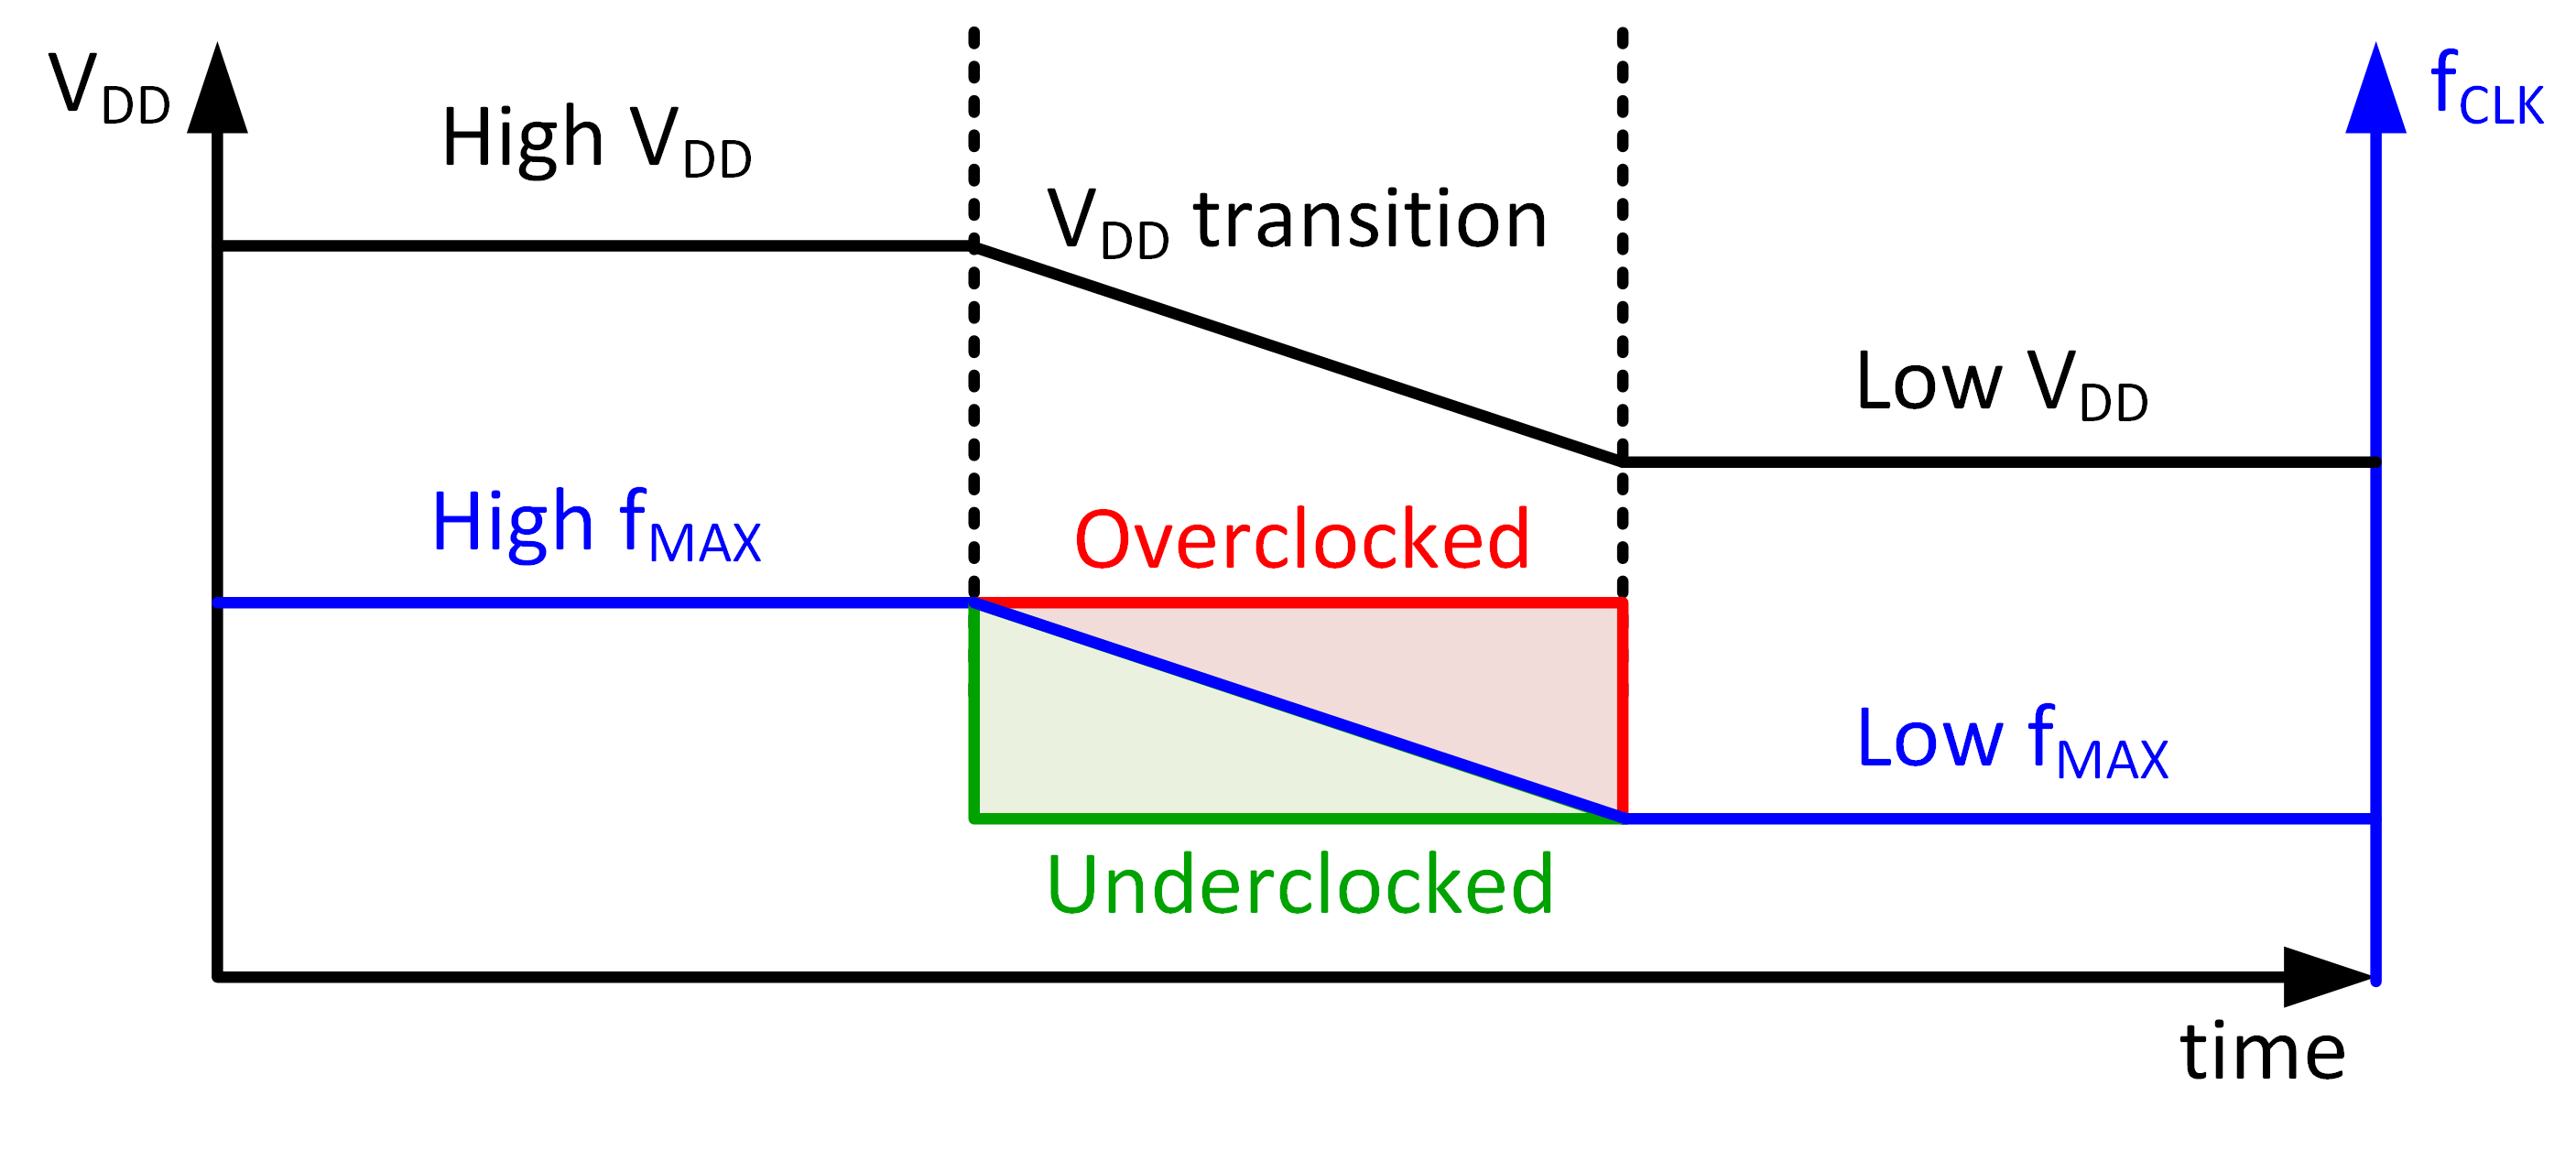
\includegraphics[width=0.85\columnwidth]{fig_fmax}
%	\caption{Reduction of $V_{DD}$ and corresponding reduction in $f_{MAX}$ (adapted from \cite{ahmad2017}).}
%	\label{fig:fmax}
%\end{figure}
\begin{figure}[h]
	\centering
	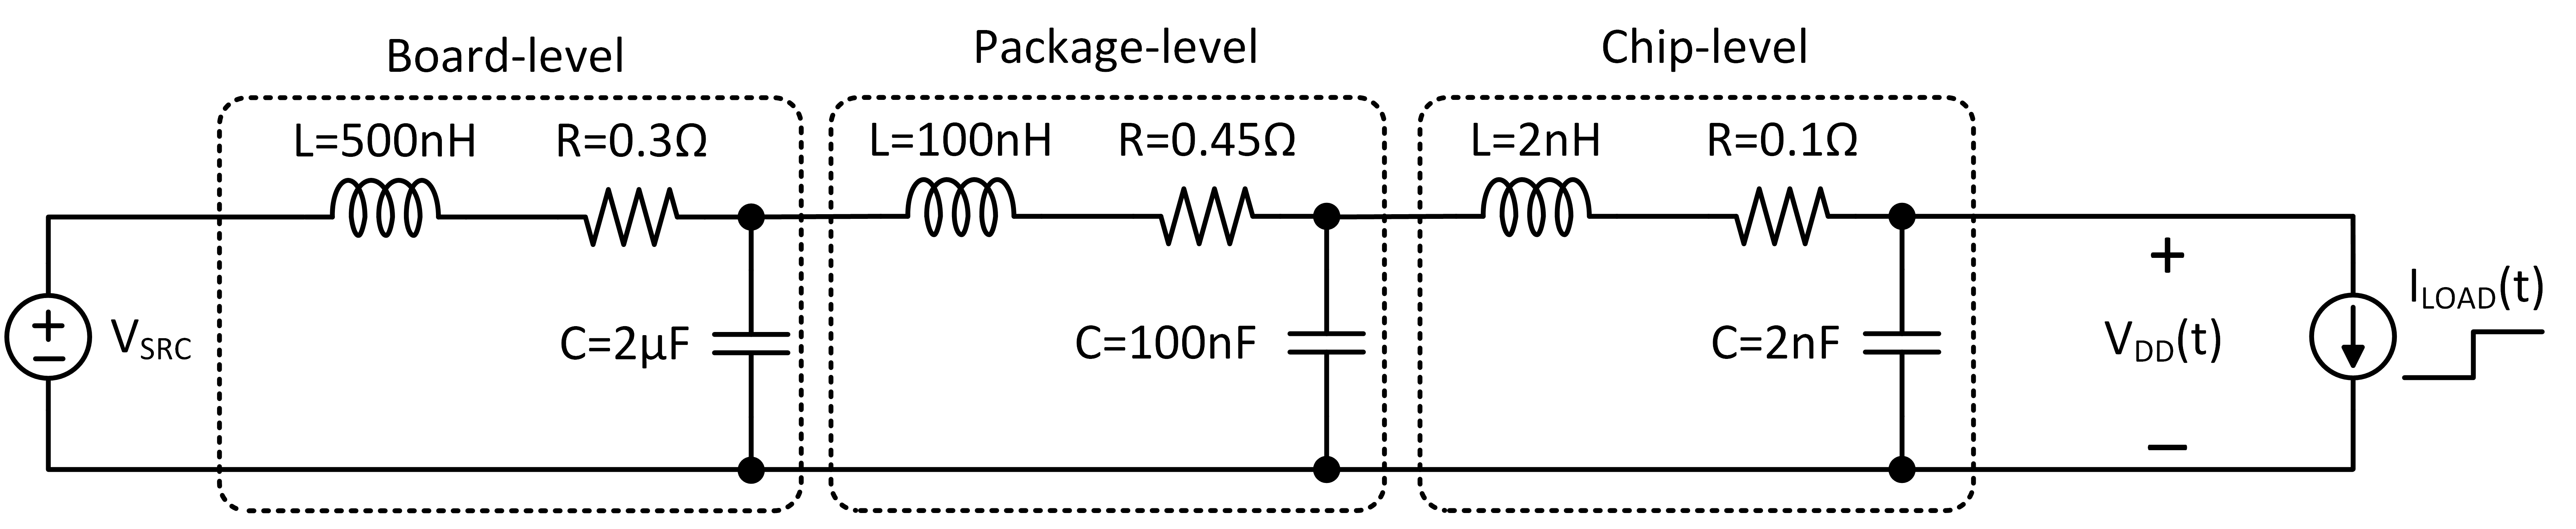
\includegraphics[width=\columnwidth]{fig_droop_schem}
	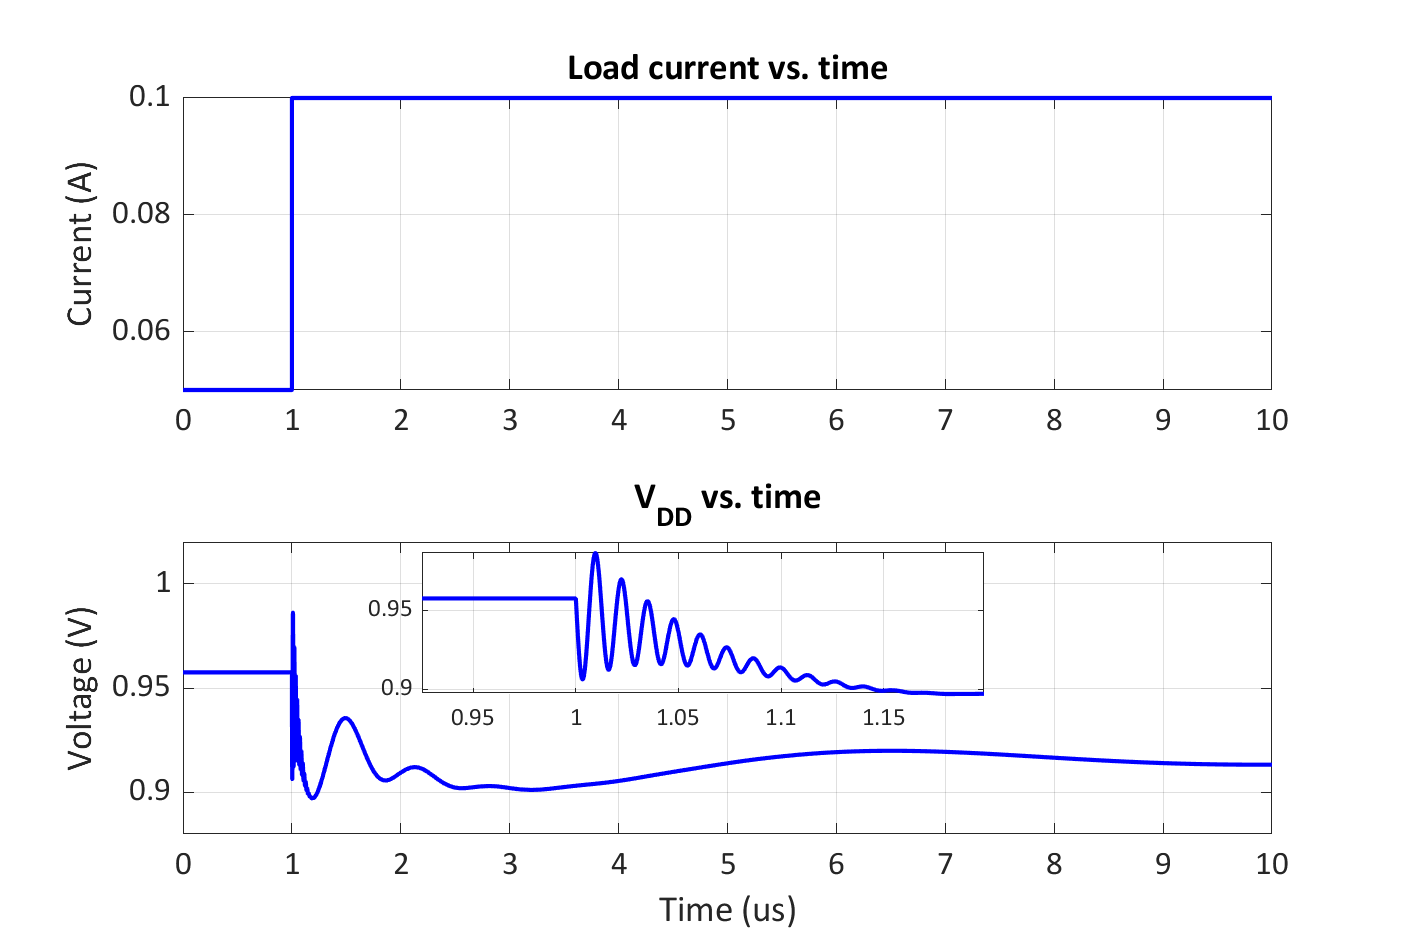
\includegraphics[width=\columnwidth]{fig_droop}
	\caption{Supply droop transients due to package inductances and load current (adapted from \cite{hashimoto2018}).}
	\label{fig:droop}
\end{figure}

To mitigate such failures, adaptive clock generation techniques have emerged in recent generations of high-performance SoCs\cite{ahmad2017,hashimoto2018,wilcox2015,floyd2017,bowman2016}. Adaptive-clock systems detect transient supply events and dynamically adjust clock frequencies to not exceed a changing $f_{MAX}$ as $V_{DD}$ decreases. %As Fig.\ \ref{fig:fmax} illustrates, a decrease from high to low $V_{DD}$ to save power corresponds to a decrease in $f_{MAX}$, and the SoC clock frequency ($f_{CLK}$) must track this change without exceeding the correct $f_{MAX}$ (overclocking) and with minimal guardbanding (underclocking) to minimize processing throughput loss during this change\cite{ahmad2017}. 
Transient response of adaptive clock techniques is vital. The external package routes supplying power to the SoC impact supply voltage settling during changes to on-chip core utilization \cite{hashimoto2018}, as illustrated in Fig.\ \ref{fig:droop}. The range of inductances \& capacitances in this network induces a medley of fast and slow time constants. Resilient adaptive clock generation circuits react quickly to fast ripples in $V_{DD}$ ranging from 50-100MHz \cite{hashimoto2018,wilcox2015} while also tracking slower transient settling at 1MHz and below \cite{hashimoto2018,bowman2016,wilcox2015}.

Several schemes exist to realize supply-induced clock adaptation ranging from directly controlling the clock-synthesizing phase-locked loop (PLL)\cite{ahmad2017,hashimoto2018} to modulating a tunable delay line or phase rotator downstream in an adaptive clock distribution (ACD) network\cite{bowman2016,floyd2017,wilcox2015,kwak2016self}. In this work, we survey and contrast the adaptive PLL- and ACD-based mechanisms presented in \cite{hashimoto2018} and \cite{wilcox2015}, respectively. This brief is organized as follows: Section \ref{sec:overview} provides an overview of adaptive clocking schemes and defines the scope of this work; Section \ref{sec:details} discusses the operating principles of mechanisms presented in \cite{hashimoto2018} and \cite{wilcox2015}; Section \ref{sec:comparison} provides a comparison of \cite{hashimoto2018} and \cite{wilcox2015}; and finally Section \ref{sec:conclusion} discusses planned work and concludes this brief.

% If using pudid, place pubidadjcol so it lands in second column of first page
\IEEEpubidadjcol

\section{Adaptive Clocking Schemes}
\label{sec:overview}

Adaptive clocking systems include two fundamental components:

\begin{enumerate}[(a)]
\item a \textit{power-supply sensor}, which measures and
reports transient droops in supply voltage; and
\item a \textit{clock period actuator}, which modulates the
system clock period in response to reports from
the power-supply sensor.
\end{enumerate}

During a supply drop, low-latency sensing and actuation is crucial to detect and adjust the clock frequency quickly to ensure error-free operation continues throughout the event. If and when $V_{DD}$ recovers from this event to its nominal value, additional circuitry can assist with managing the corresponding $f_{CLK}$ recovery.

ACD- and adaptive PLL-based systems differ in their implementation of the clock period actuator. ACD-based systems decrease the clock frequency by extending clock periods using an ACD circuit placed between the clock-synthesizing PLL and the global clock distribution network as illustrated in Fig.\ \ref{fig:overview_acd}. A digital code $CTRL_{FCLK}$ from the power supply sensor controls the ACD circuit such that it extends the period of the synthesized clock, $CLK_{PLL}$, to the desired frequency given the sensed change in $V_{DD}$. This lower-frequency clock, $CLK_{SOC}$, is then distributed through the global clock network to the SoC processing cores. Examples of this ACD circuit include tunable-length delay \cite{bowman2016} and phase rotators \cite{wilcox2015}, of which the latter is discussed in Section \ref{sec:details_acd}.

\begin{figure}[h]
	\centering
	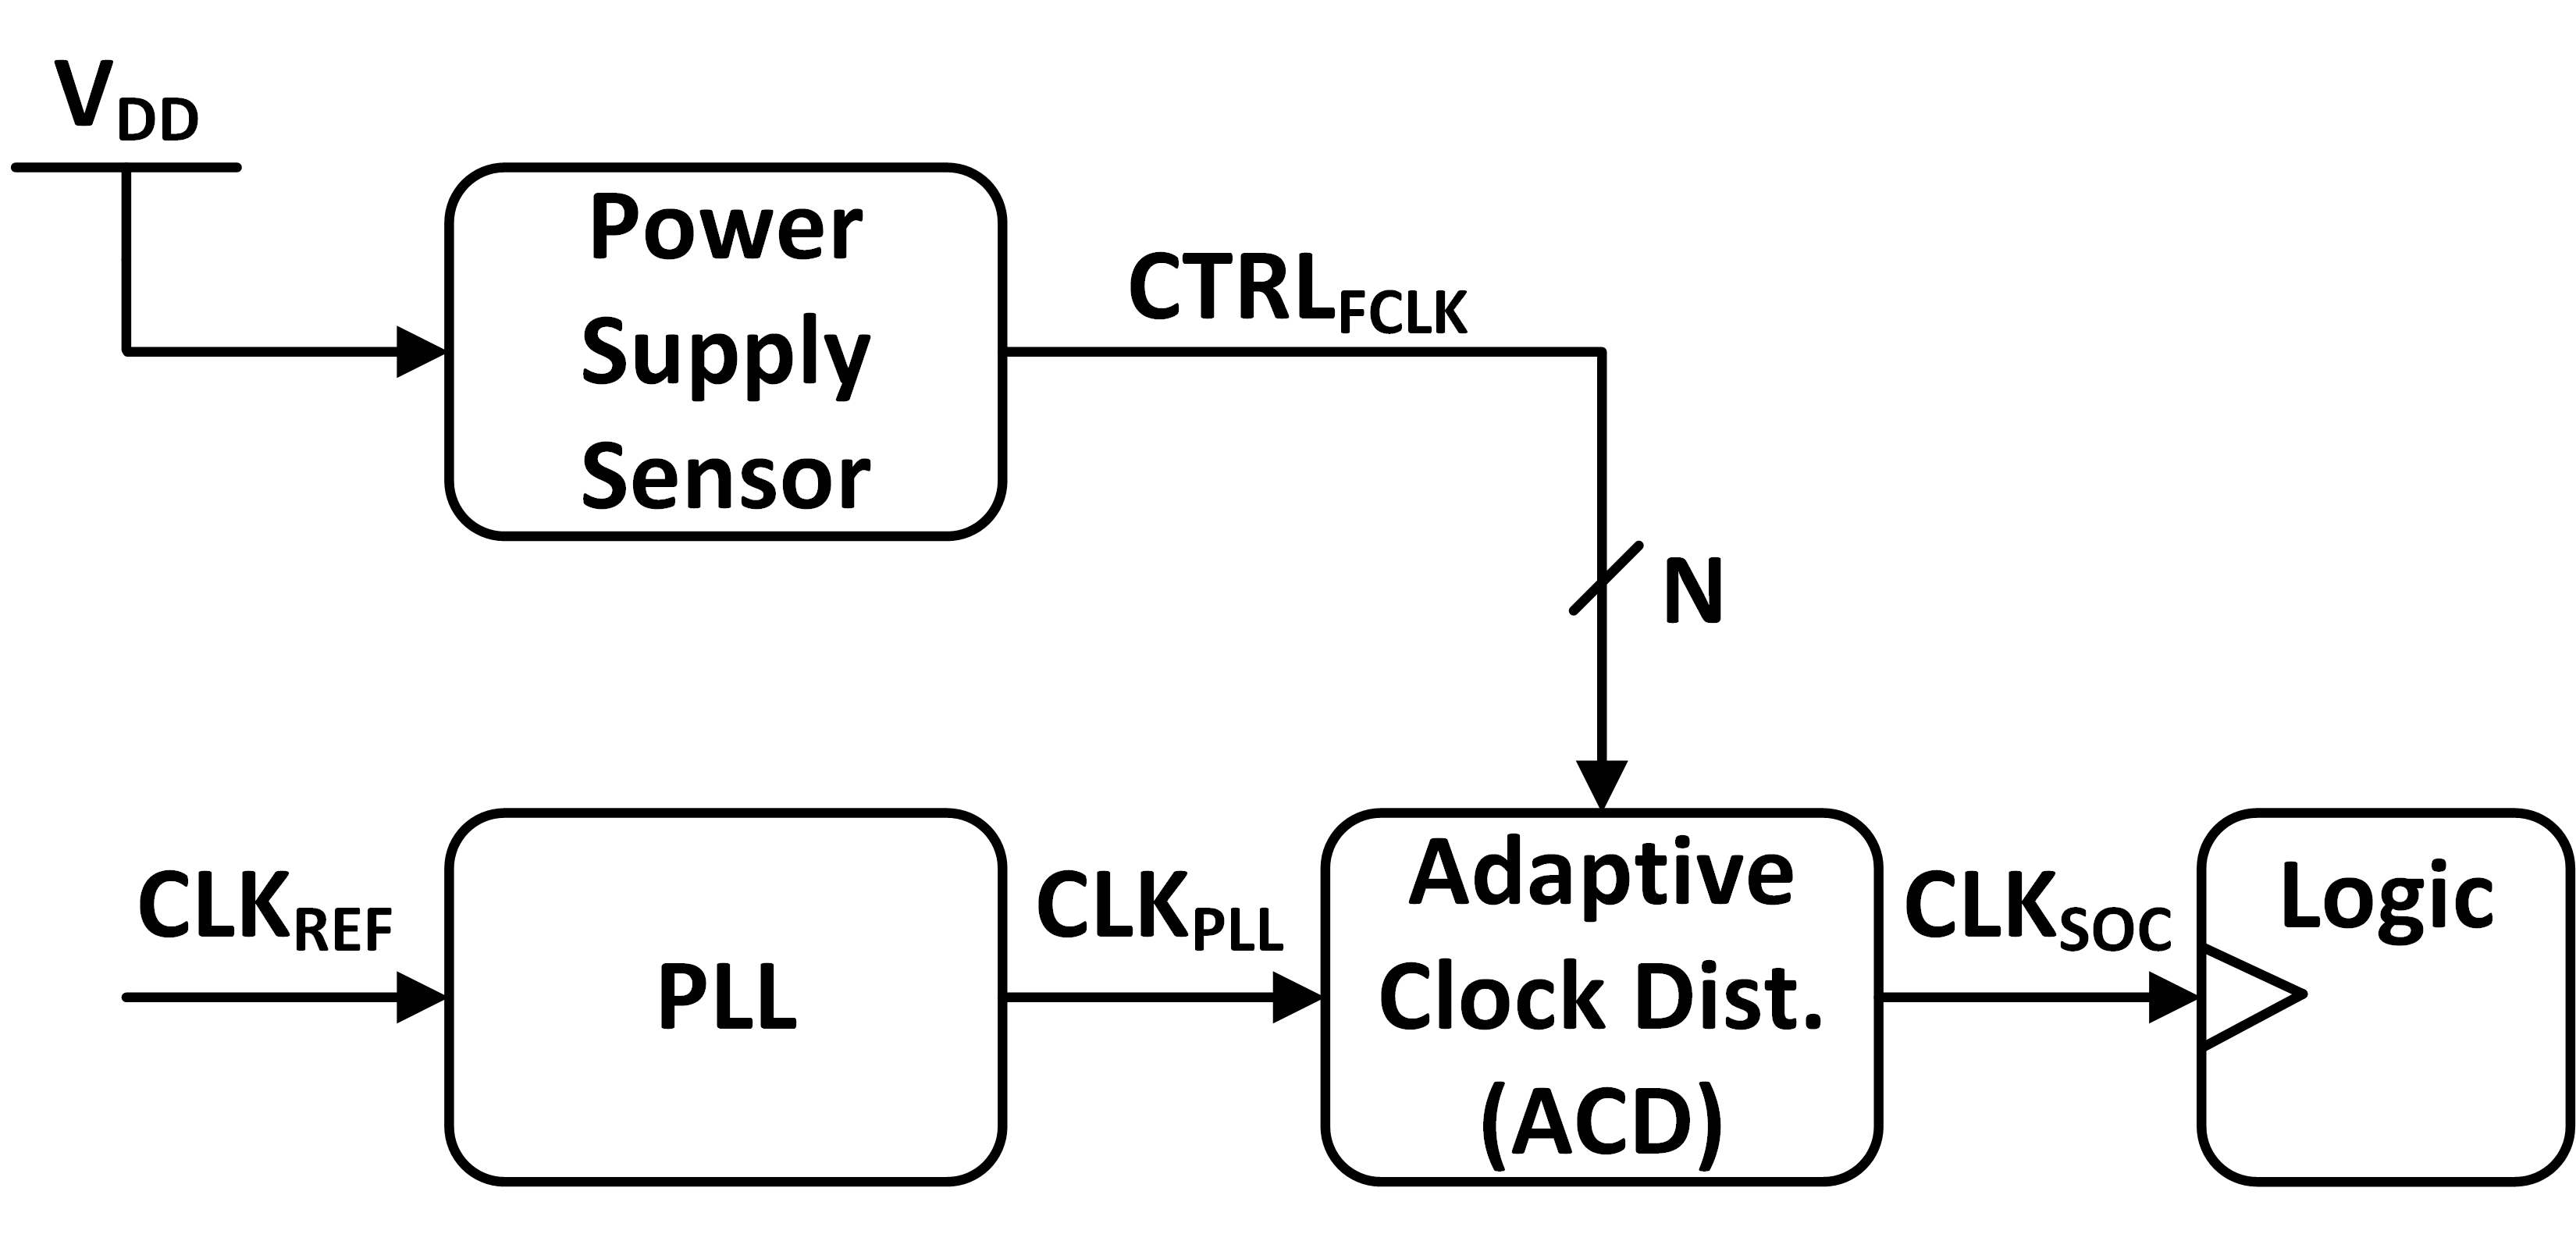
\includegraphics[width=0.7\columnwidth]{fig_overview_acd}
	\caption{Adaptive clock distribution (ACD) based system.}
	\label{fig:overview_acd}
\end{figure}

\begin{figure}[h]
	\centering
	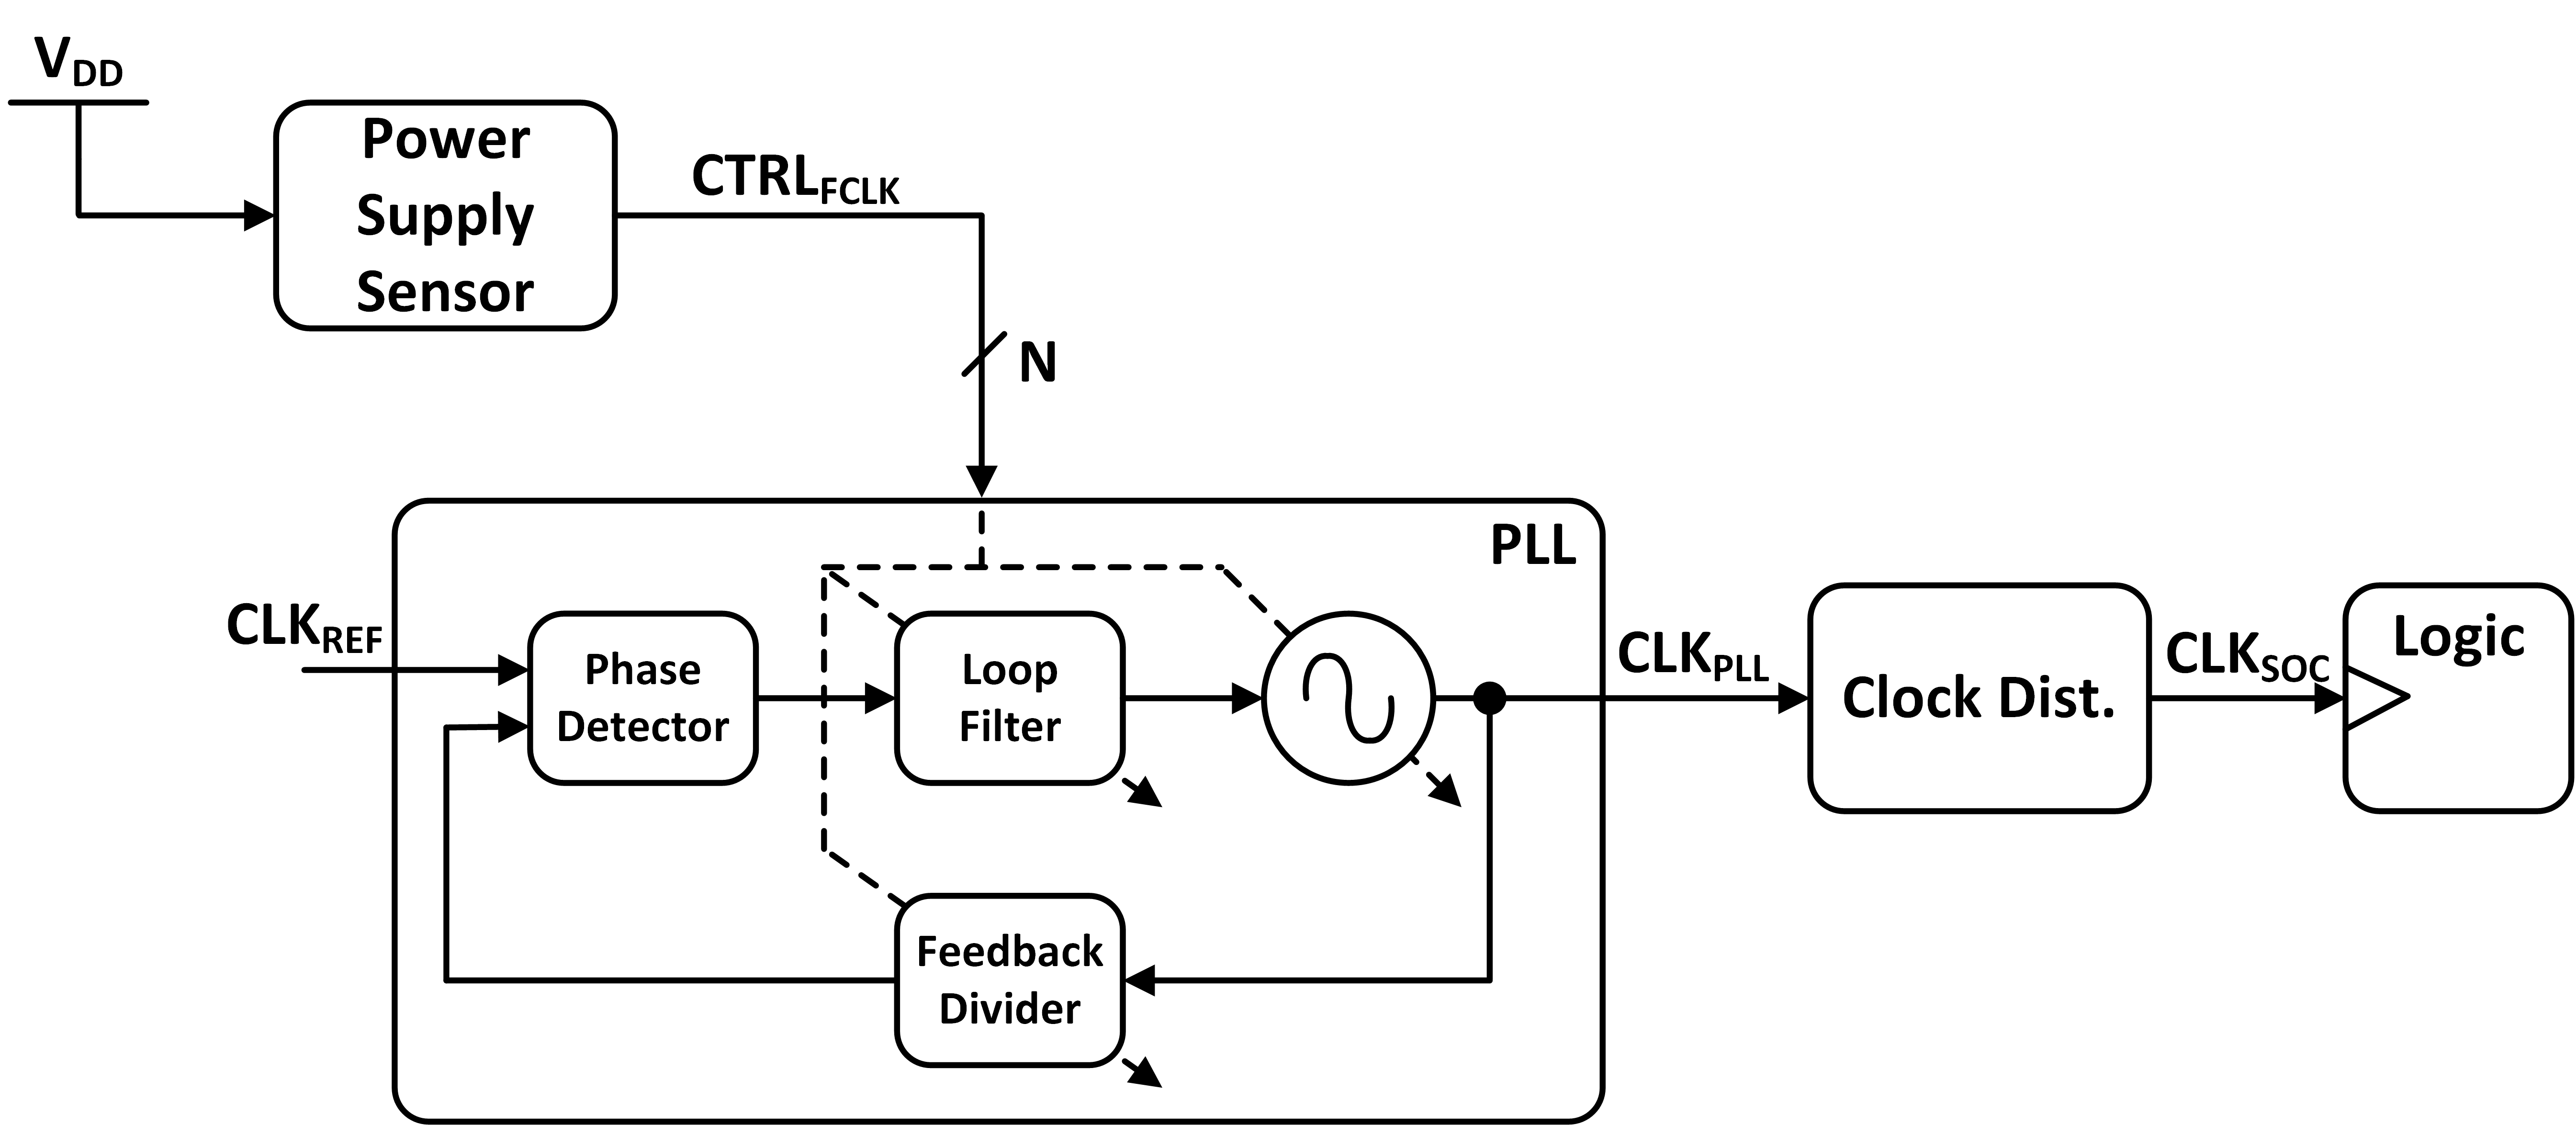
\includegraphics[width=\columnwidth]{fig_overview_pll}
	\caption{Adaptive PLL-based system with possible intra-PLL control variants.}
	\label{fig:overview_pll}
\end{figure}

Adaptive PLL-based systems, in contrast, incorporate information from the power-supply sensor to dynamically change the behaviour of PLL sub-components. Typically, these schemes affect oscillator control on top of the traditional PLL loop. In \cite{ahmad2017} for example, the oscillator is controlled indirectly through a loop filter modified for droop response: when a droop is detected, the traditional proportional- and integral-loop filter switches to proportional-only to form a type-I PLL that tunes the oscillator to frequency lock without hazardous over- or underclocking. In \cite{hashimoto2018}, this idea is further extended by interrupting the PLL feedback loop to modify the oscillator directly, reacting to a supply droop event with relatively low latency. The feedback divider is then slowly modified to restore PLL lock. This latter work is further discussed in Section \ref{sec:details_pll}.

The focus of this brief is to compare the design and effectiveness of clock period actuators in ACD and PLL-based schemes. While high-resolution power-supply sensors and their low-latency integration are critical to the overall adaptation time of such schemes, it remains beyond the scope of this work.

\section{Operating principles}
\label{sec:details}
The two main works for comparison are the PLL- and ACD-based adaptive clocking schemes in \cite{hashimoto2018} and \cite{wilcox2015} respectively. The operating principles of each are described in this section.

\vspace{-10pt}
\subsection{PLL-based adaptive clocking}
\label{sec:details_pll}
The scheme reported in \cite{hashimoto2018} presents a PLL-based adaptive clocking control for three SPARC processor cores in a 20nm CMOS testchip. A sense point placed near one of the SPARC cores transmits the core $V_{DD}$ through low-impedance on-package (off-chip) routing to the on-chip power-supply sensor. This sensor converts $V_{DD}$ droops into a thermometer-coded quantized digital signal, $q[n]$, by use two calibrated delay lines and a 8-bit time-to-digital converter (TDC). 

A major contribution of \cite{hashimoto2018} is to use the instantaneous value of q[n] to immediately reduce the PLL's oscillator frequency to correct for high-frequency droops and use a filtered version of $q[n]$ to correct for low frequency droops and ultimately re-lock the PLL feedback loop. As shown in Fig.\ \ref{fig:detail_pll}, %and Fig.\ \ref{fig:detail_pllarch}, 
$q[n]$ is processed by the frequency control logic to generate two control signals: $\Delta F_{code}$ that can instantaneously respond to changes in $q[n]$ to directly change the digitally-controlled oscillator (DCO) frequency, and $N^{sync}_{code}$ that relies only on a filtered value of $q[n]$ to track low-frequency droops and re-lock the PLL loop at the new frequency by changing the feedback division value. The minimum function and the non-linear filter together effectively construct an all-pass filter when $V_{DD}$ decreases and a low-pass filter when $V_{DD}$ increases. They allow the loop to actuate the clock with minimal latency during a $V_{DD}$ droop event. During droop recovery, they low-pass filter $V_{DD}$ transients and overshoots as the voltage ultimately settles to its nominal value.

\begin{figure}[h]
	\centering
	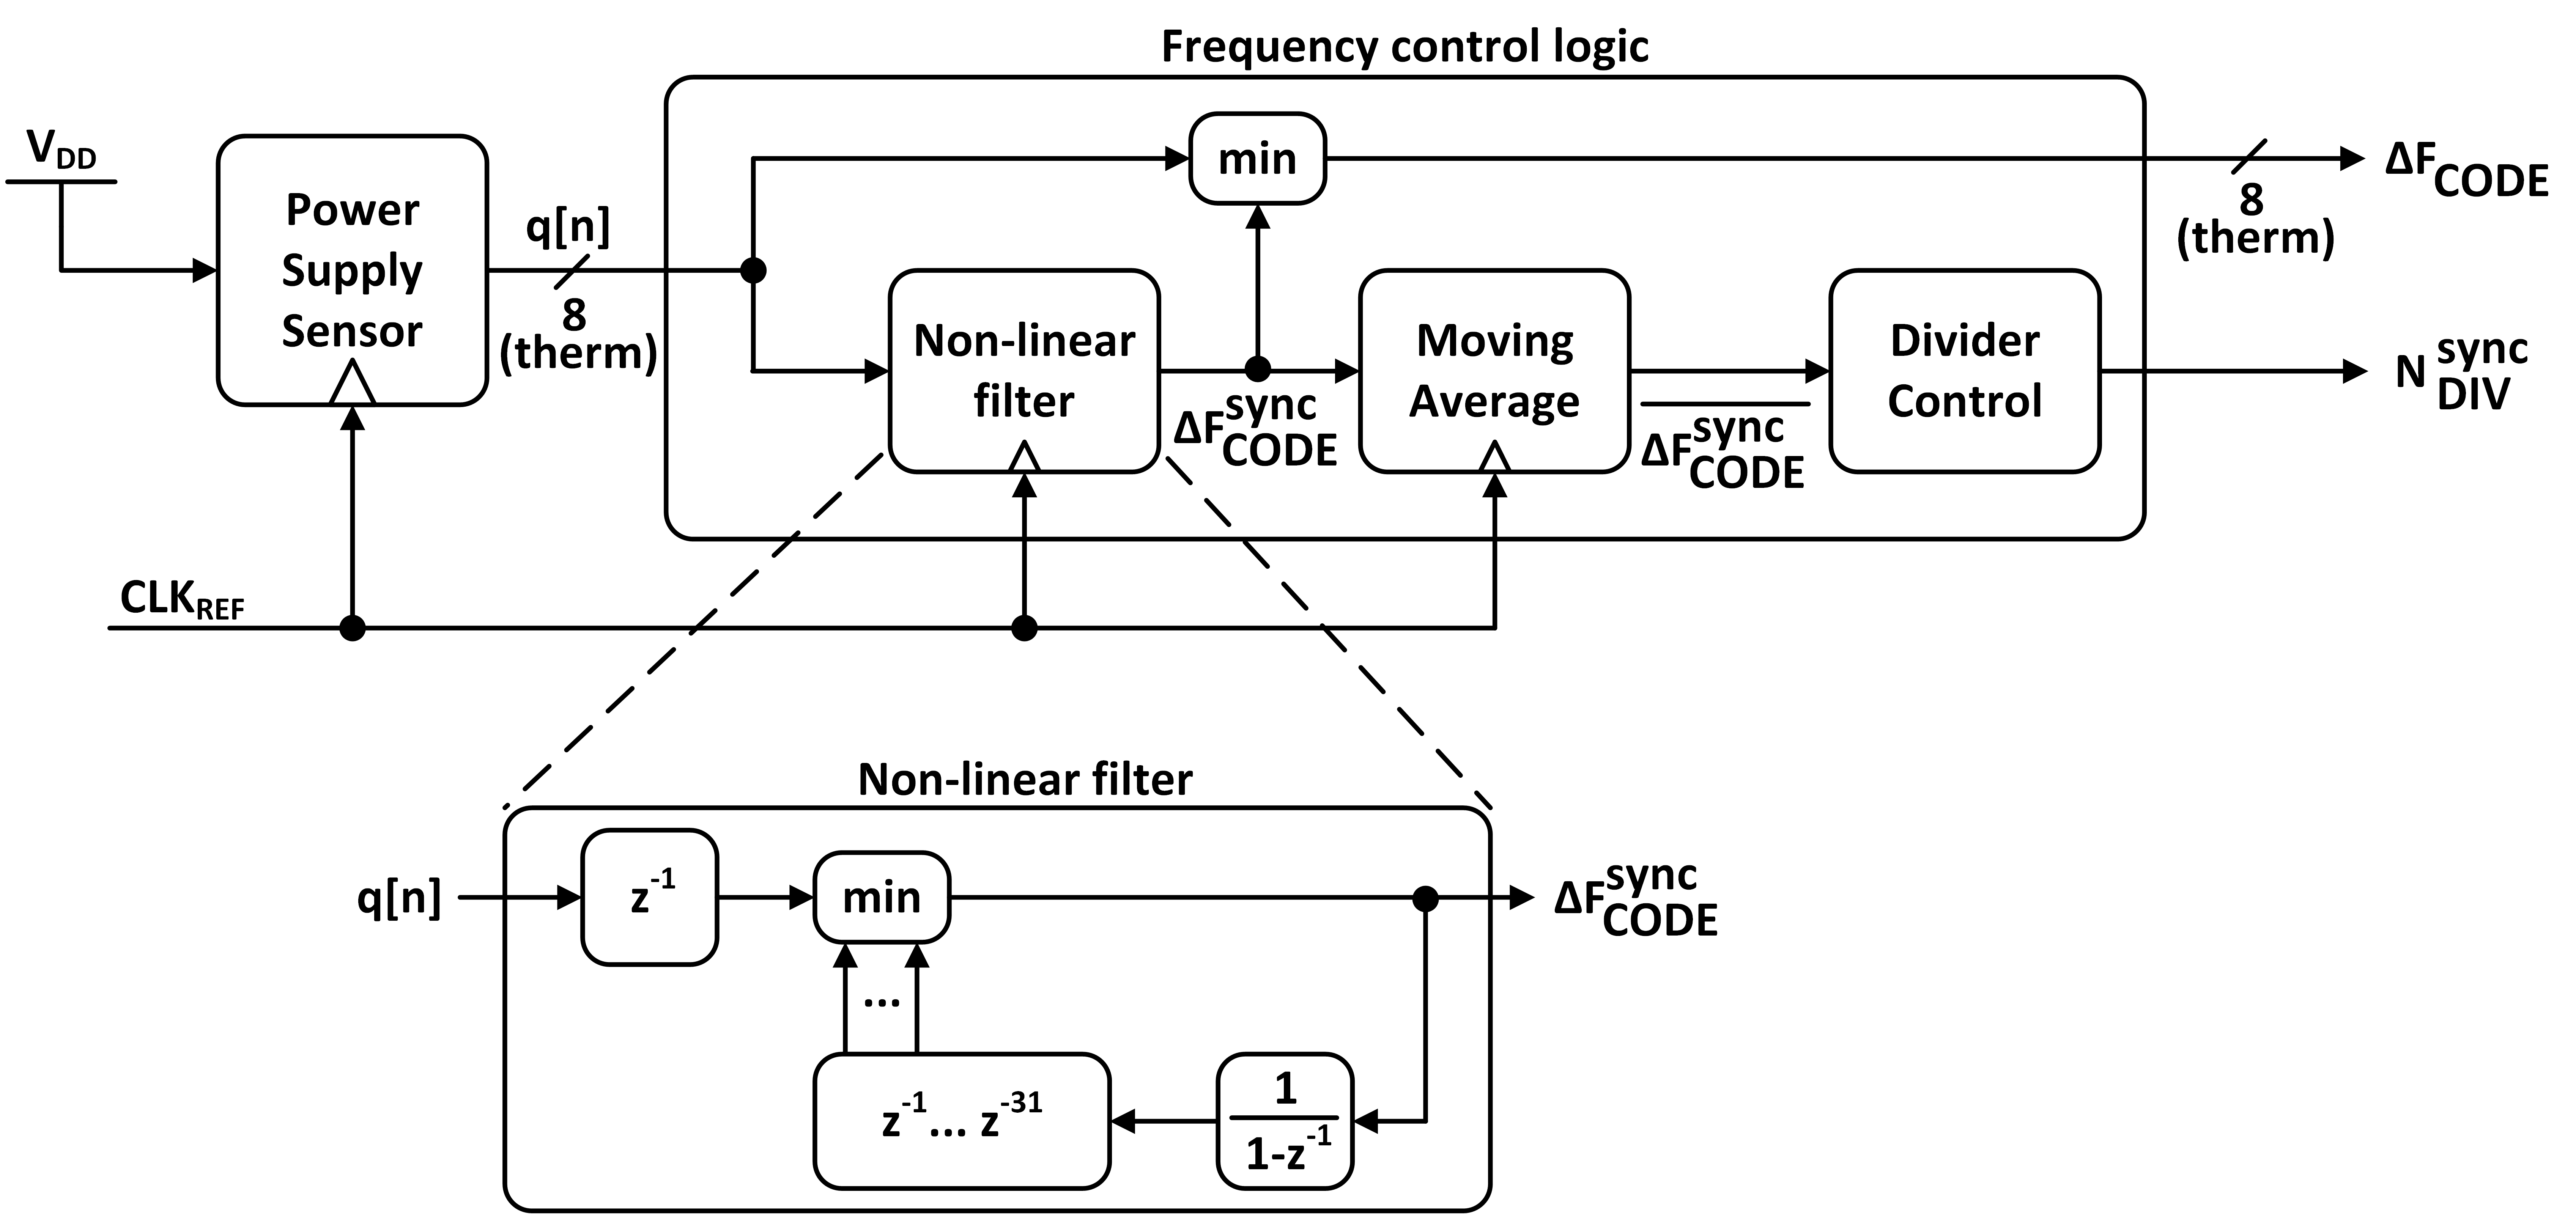
\includegraphics[width=\columnwidth]{fig_detail_pll}
	\caption{Frequency control logic for PLL-based adaptive clocking in \cite{hashimoto2018}.}
	\label{fig:detail_pll}
\end{figure}

%\begin{figure}[h]
%	\centering
%	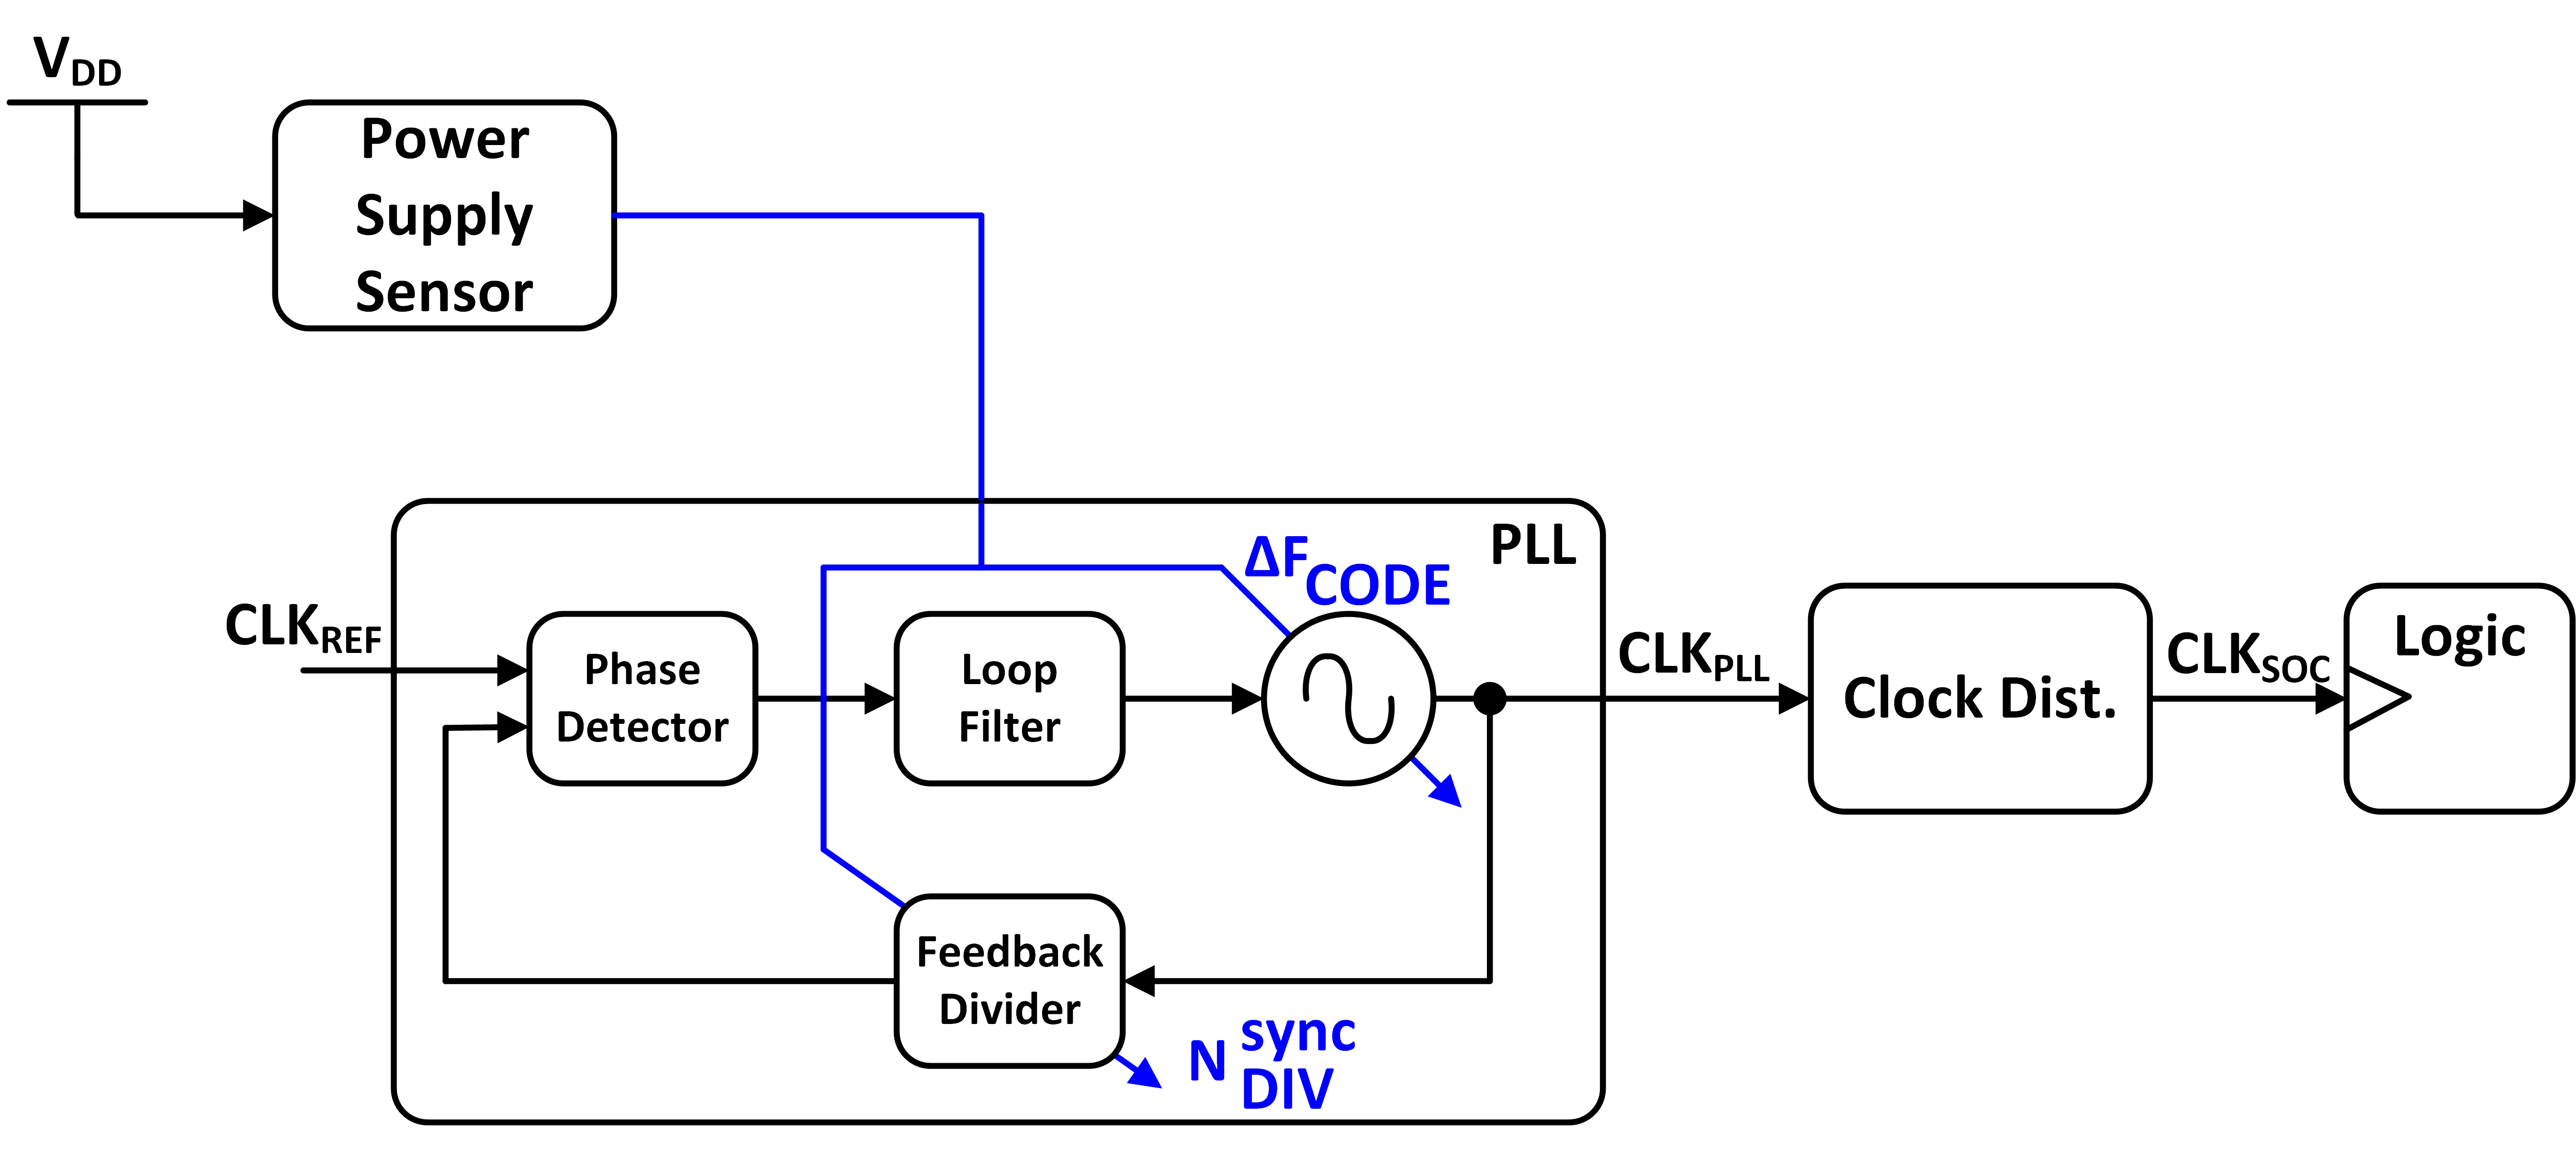
\includegraphics[width=\columnwidth]{fig_detail_pllarch}
%	\caption{Intra-PLL control for PLL-based adaptive clocking in \cite{hashimoto2018}.}
%	\label{fig:detail_pllarch}
%\end{figure}

A fast response to high-frequency supply droops is an important criterion in \cite{hashimoto2018}, significant design efforts were made to ensure low-latency clock period actuation. The reported design target is 8$\times$ faster than the first-droop frequency of 50MHz. This permits a time window of 2.5ns from the time $V_{DD}$ crosses the first supply sensor threshold to the time the SoC clock frequency is corrected. This narrow timing constraint is met by generating and propagating the critical oscillator control signal $\Delta F_{code}$ asynchronously. Crucially, the 8-bit thermometer-coded $\Delta F_{code}$ controls a DCO that can tolerate asynchronous changes in its code without glitching its output clock. The DCO reported in \cite{hashimoto2018} is a bank of nine ring inverters with eight of the rings independently enabled by each thermometer bit of $\Delta F_{code}$. Such a structure can tolerate asynchronous arrival of $\Delta F_{code}$ when suddenly decreasing frequency, as the case of a droop. Note that frequency increases are restricted: the combination of non-linear filter memory with the masking of minimum function ensures $\Delta F_{code}$ only increases one bit at a time after droop recovery \cite{hashimoto2018}. This obviates synchronization of $\Delta F_{code}$, reducing adaptation latency.

The reduction in adaptation latency directly correlates with reported experimental results. Fast response to droops allows for tighter guardbanding and therefore higher $f_{MAX}$. While \cite{hashimoto2018} does not report the exact clock adaptation latency, the work improves $f_{MAX}$ by 7.5\%, from 4.65GHz without adaptive clocking to 5.00GHz with the proposed scheme. This is the largest frequency gain reported in compared works.

\vspace{-10pt}
\subsection{ACD-based adaptive clocking}
\label{sec:details_acd}
The scheme reported in \cite{wilcox2015} presents a ACD-based adaptive clocking control for AMD's Steamroller CPU in 28nm CMOS. The power supply sensor consists of a DLL-based droop detector acting as a delay line connected to the SoC core $V_{DD}$: as $V_{DD}$ changes, the DLL phases change with respect to a regulated PLL's output clock. A programmable threshold selects one of four DLL phases to compare against the reference PLL phase to signal a 1-bit droop activity.

Fig.\ \ref{fig:detail_acd} illustrates the reported scheme. A DLL-based phase rotator realizes the ACD circuit. When a droop activity is detected and $DroopDetected$ is asserted, phase rotation between the 40 DLL phases occurs to effectively ``stretch" the clock period and reduce the clock frequency. To ensure glitchless phase rotation, small positive pre-programmed phase increments occur at each step, and the phase rotator rotates through all 40 phases before continuing the cycle. Rotation can be bypassed entirely by de-asserting $DroopEnable$. 

\begin{figure}[h]
	\centering
	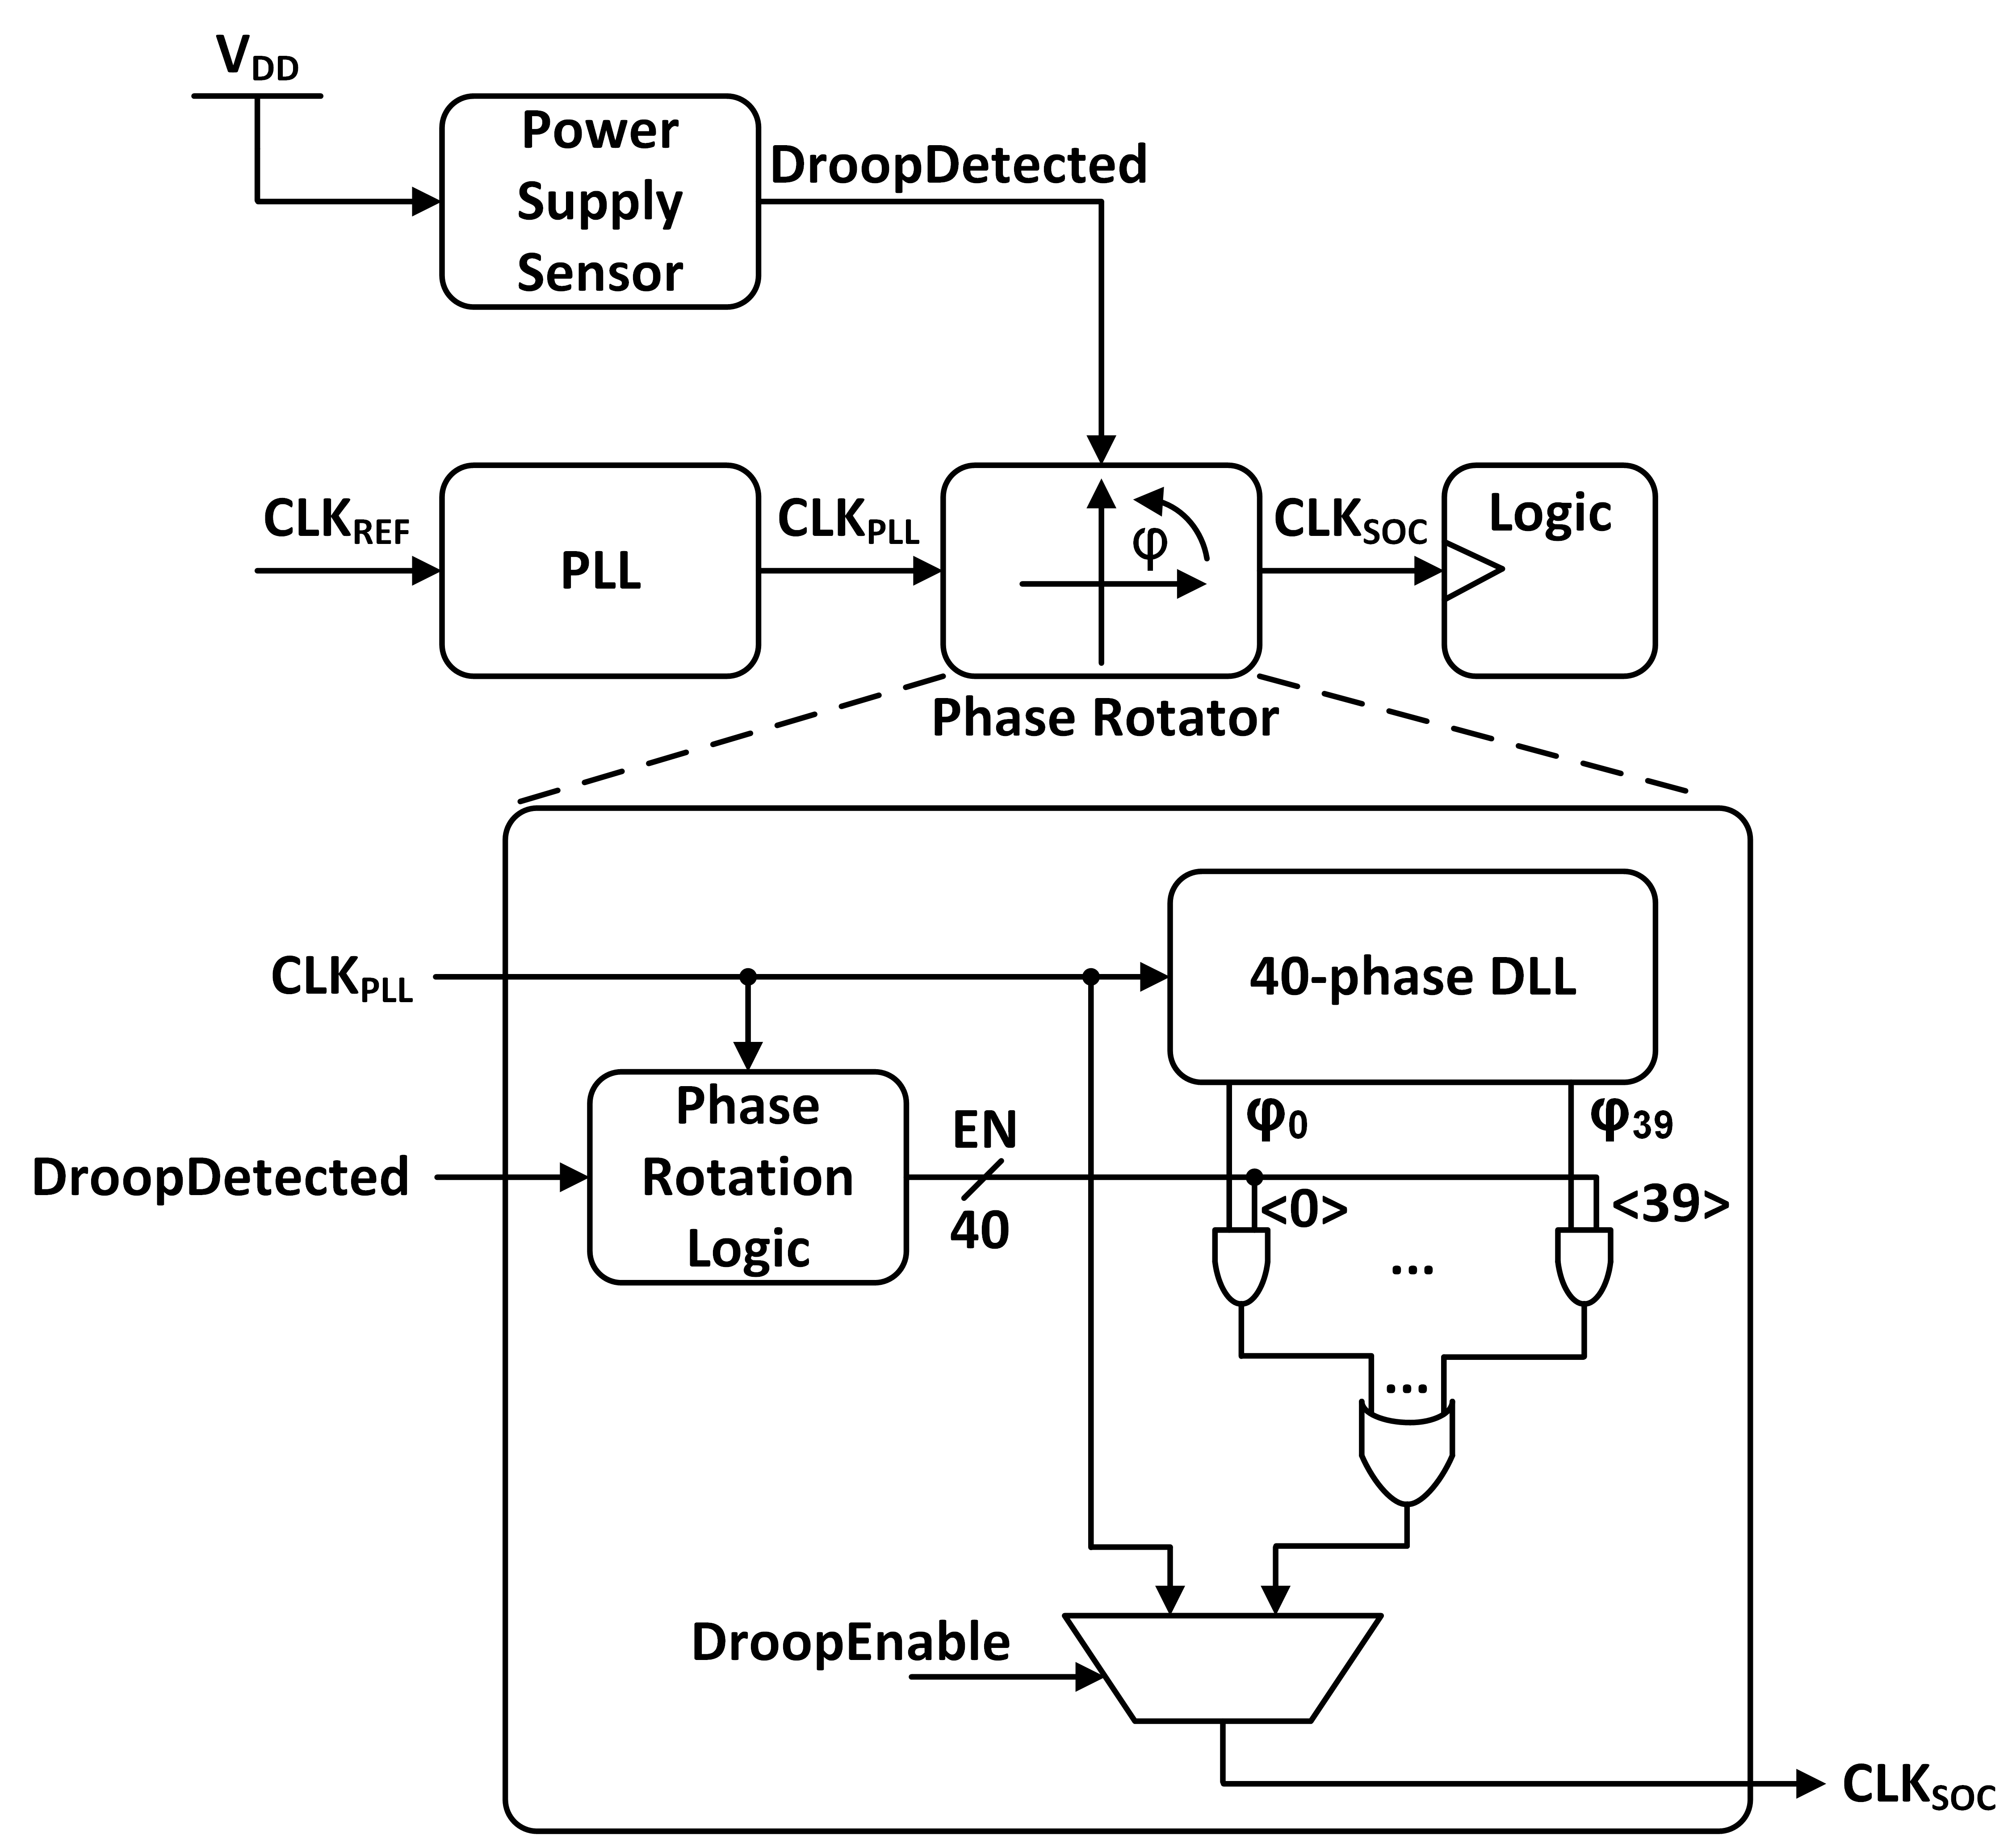
\includegraphics[width=0.7\columnwidth]{fig_detail_acd}
	\caption{Frequency control logic for ACD-based adaptive clocking in \cite{wilcox2015}.}
	\label{fig:detail_acd}
\end{figure}

This scheme reports to target fast initial droops of 100MHz and slower 1-5MHz secondary droop transients by means of the programmed droop detector threshold \cite{wilcox2015}. As the detector signal is binary, the ACD-based reduces the SoC clock frequency by a fixed amount (phase rotator steps through a fixed phase step per cycle) or does not change the frequency at all. Voltage recovery is triggered when $V_{DD}$ crosses back beyond the detector threshold. The work reports a total adaptation latency of 3 cycles at 3.4GHz from droop detection to clock frequency reduction. While experimental results do not report frequency gain as in \cite{hashimoto2018}, silicon results demonstrated a reduction of 3-6\% in $V_{MIN}$, the minimum supply voltage tolerable at a given frequency for the SoC. No comparison was provided with prior works.

\section{Comparison of ACD and PLL Actuators}
\label{sec:comparison}

\subsection{Comparison Scope}
\label{sec:Scope of comparison}

As discussed in Section \ref{sec:overview}, clock adaptation consist of various sub-components and their latencies. This is illustrated in Fig.\ \ref{fig:scope}. Design of a complete adaptation system requires a $V_{DD}$ sense point, routing delay, detector and actuation latencies, and finally clock propagation delay. This comparison focuses on the detection logic, clock actuation, and their combined actuation latency. There are indeed important specifications beyond this when designing adaptation circuits. For example, sensor resolution, bandwidth, and ease of design integration with digital SoCs are important considerations: highly digital sensors \cite{hashimoto2018,wilcox2015} to custom analog voltage mixing \cite{kurd2009} have their bandwidth and integration tradeoffs. However, the scope of this comparison focuses on PLL- and ACD-based adaptive clocking presented in \cite{hashimoto2018} and \cite{wilcox2015} respectively, agnostic to extraneous design considerations.

\begin{figure}[h]
	\centering
	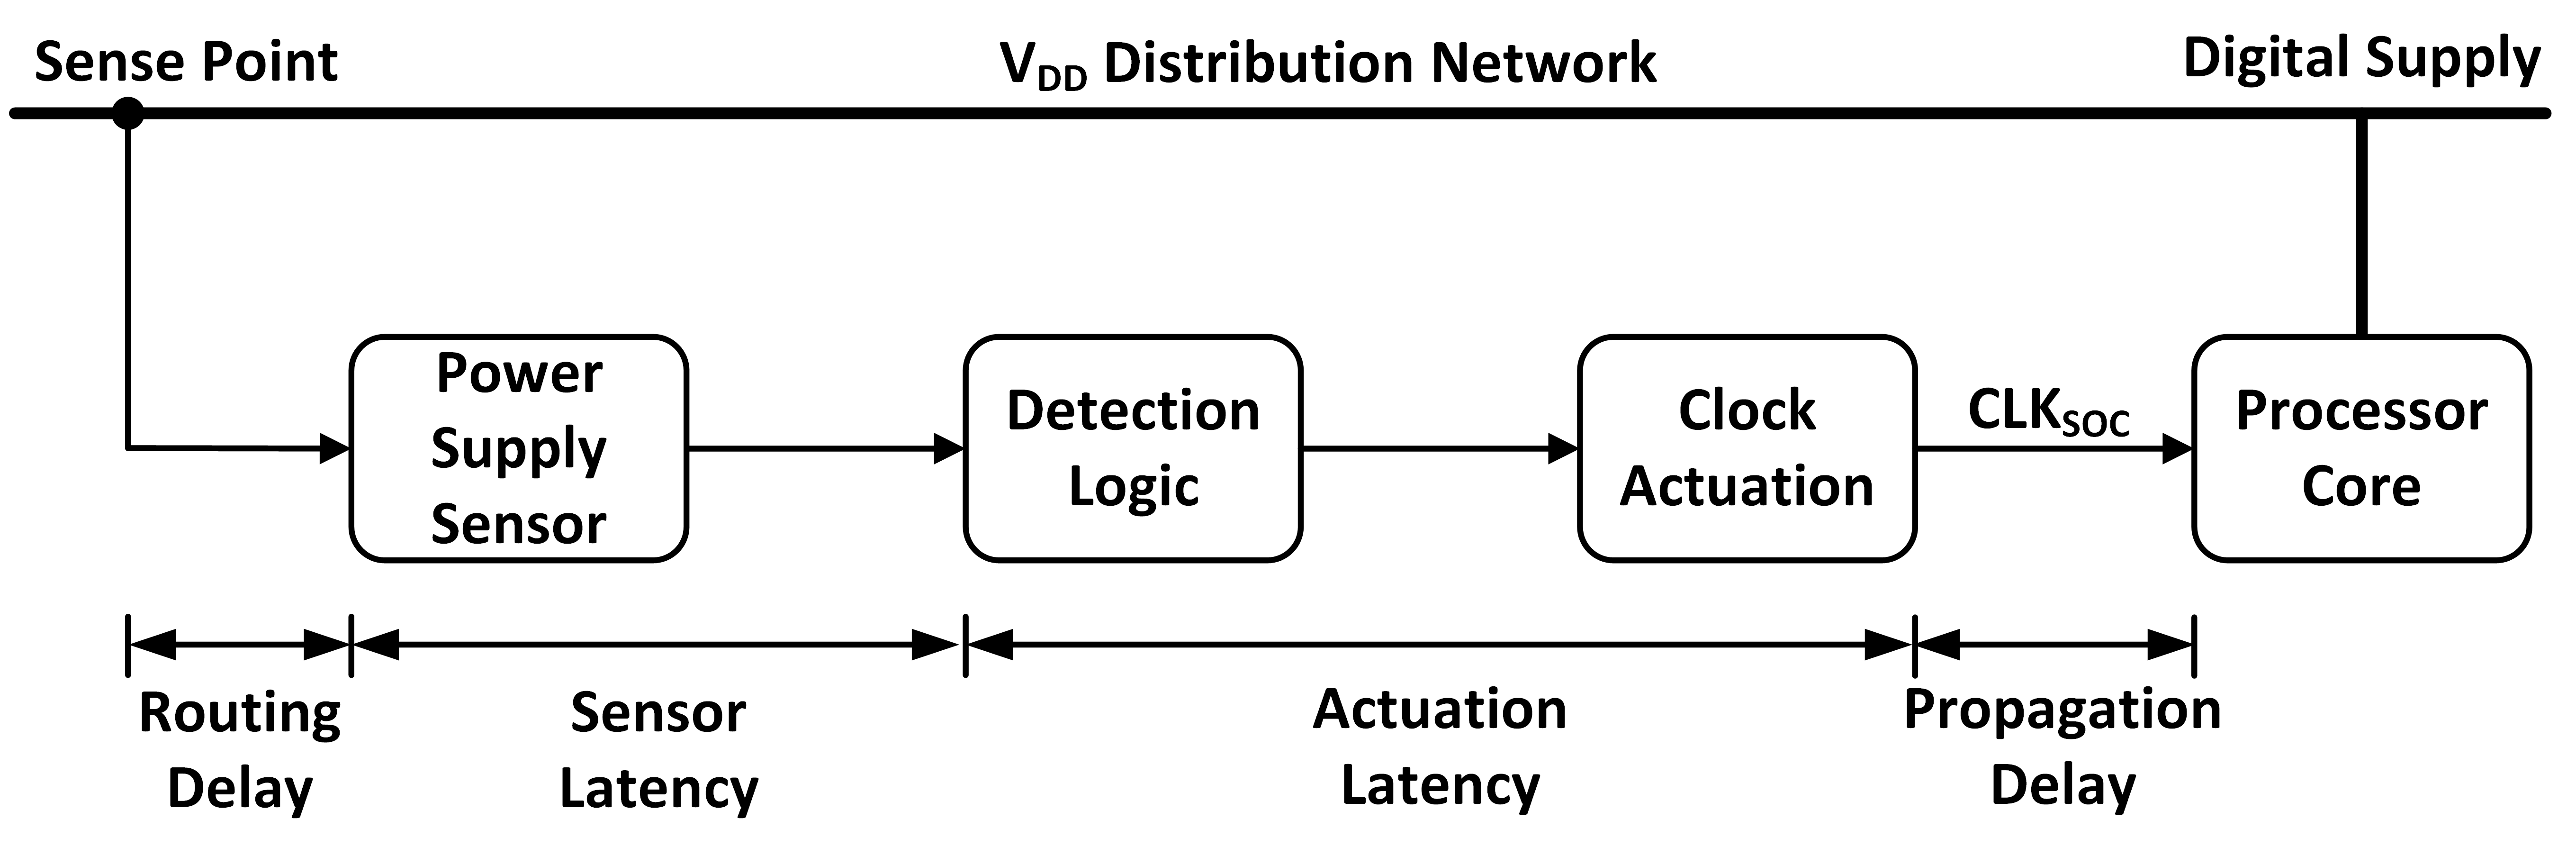
\includegraphics[width=\columnwidth]{fig_scope}
	\caption{Various latencies in adaptive clock system (adapted from \cite{hashimoto2018}).}
	\label{fig:scope}
\end{figure}

In comparing the PLL- and ACD-based adaptive clocking schemes, key metrics are identified: actuation latency, power/area, calibration, and frequency gain/$V_{MIN}$ reduction. Forecasts for these metrics in the predictive 7nm technology ASAP7 \cite{asap7} are also discussed.

\vspace{-10pt}
\subsection{Actuation Latency}
\label{sec:ActuationLatency}
Minimizing actuation latency helps reduce overall system response time. In \cite{hashimoto2018}, the PLL-based actuation latency varies depending on the direction of $V_{DD}$ change due to the non-linear adaptation filter. As previously discussed, for decreases in $V_{DD}$, the latency is less than one clock cycle and limited by asynchronous propagation delay through the minimum function in Fig.\ \ref{fig:overview_pll} and the control bandwidth of the oscillator. The control port time constant is approximately $\frac{T_{VCO}}{2N}$ for the reported oscillator \cite{hashimoto2018}. Assuming the routing parasitic from the minimum logic to the oscillator control port is negligible, this allows a latency below one clock cycle at the reported $f_{MAX}$ = 5GHz, i.e. $t_{act} <$ 200ps.

Conversely, the ACD-based actuation latency is reported as 2 clock cycles at 3.4 GHz \cite{wilcox2015}, implying $t_{act} =$ 588ps. This is due to synchronizing $DroopDetected$ to the PLL clock domain  and generating the corresponding phase rotation enable signal as was shown in Fig.\ \ref{fig:detail_acd}.

We predict these results will be comparable in ASAP7. The actuation latency in \cite{wilcox2015} will remain 2 clock cycles by design. That in \cite{hashimoto2018} will remain less than one cycle again by design, with the potential for $t_{act}$ to be reduced due to increased $f_{T}$. One drawback may be higher resistance routing which could decrease oscillator control bandwidth if not carefully designed.

\vspace{-10pt}
\subsection{Power/Area}
\label{sec:power_area}
While neither works report measured power and area overhead of the actuation or overall adaptation circuits, the use of a DLL in \cite{wilcox2015} is estimated to cost more. Consider phase mismatch and jitter amplification in the DLL \cite{wilcox2015}. The 40-phase DLL consists of 20 pseudo-differential delay cells, each designed as a pair of cross-coupled inverters with tunable MOS capacitor (MOSCAP) loads. In theory, the $k^{th}$ and $(k+20)^{th}$ phases have a standard deviation of $\sqrt{k} \sigma_{u}$ where $\sigma_{u}$ is one stage's delay variation. The DLL must, at a minimum, ensure phase monotonicity to guarantee glitchless phase rotations. $\sigma_{u}$ is directly correlates to $V_{t}$ and thereby area.

%The DLL can also have power implications on the upstream PLL through system jitter specifications. Assume the DLL nears a 2$\times$ tuning range, similar of ring-based PLLs. Each DLL stage must achieve a min/max delay spread of 2$\times$. Fig.\ \ref{fig:dllasap7} shows schematic simulations in ASAP7 of an example delay stage operating at maximum $f_{CLK}=$ 3GHz. To achieve higher delay spread per stage, higher MOSCAP sizing is needed. However, this also decreases the RC bandwidth at each stage, increasing deterministic jitter amplification such as duty-cycle distortion (DCD) as also shown in Fig.\ \ref{fig:dllasap7}. To ensure jitter is not amplified through the DLL, the overall delay chain should target jitter amplification $<$ 1. Otherwise, power must be expended in the upstream PLL to reduce input jitter and DCD.

%\vspace{-10pt}
%\begin{figure}[h]
%	\centering
%	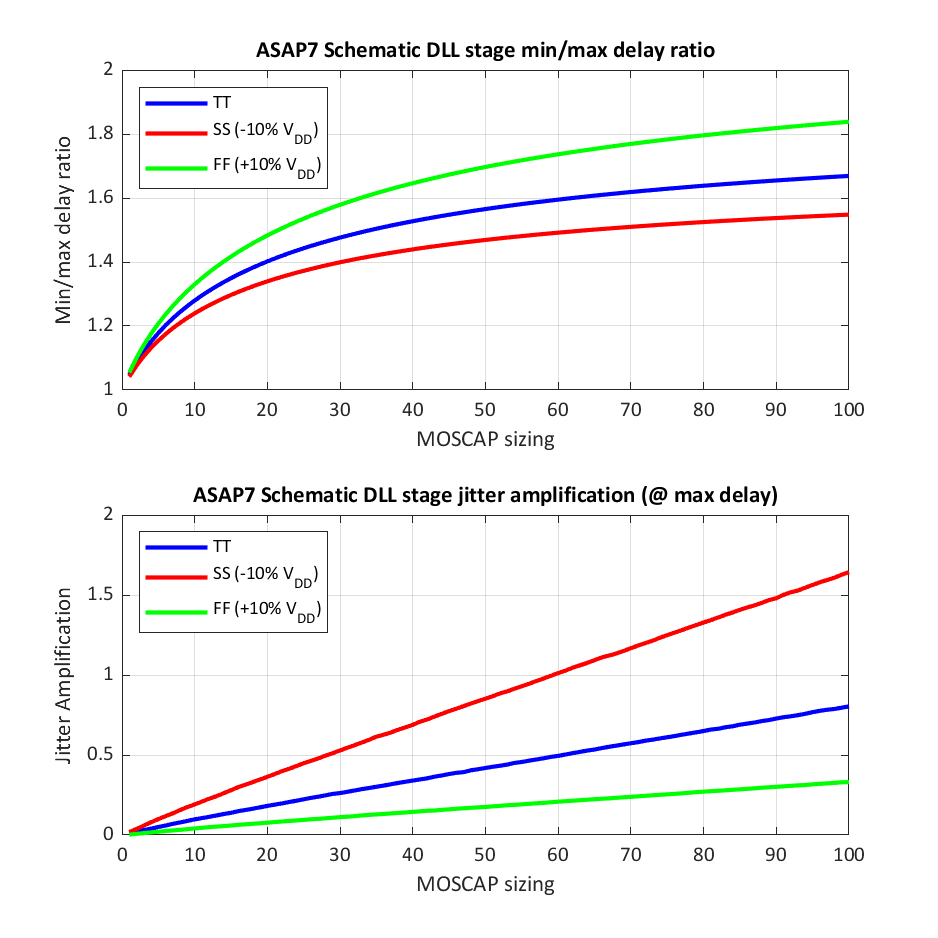
\includegraphics[width=0.8\columnwidth]{fig_dllasap7}
%	%\caption{Schematic simulation of example DLL stage in ASAP7: min/max delay ratio (top) and jitter amplification (bottom) per stage.}
%	\caption{Schematic simulation of example DLL stage in ASAP7.}
%	\label{fig:dllasap7}
%\end{figure}
%\vspace{-15pt}
%\subsection{Design \& Calibration}
%\label{sec:calibrationoverhead}
%Design-time complexity of the PLL-based scheme in \cite{hashimoto2018} involves an unconventional PLL loop, a detection filter overriding the VCO control and the restoring of PLL lock during frequency recovery by ramping the feedback divider value. Conversely, the ACD-based scheme in \cite{wilcox2015} is a simpler design that does not require modifications to a PLL, and instead inserts a phase rotator in the clock network between it and the SoC. Both works report manually calibrate supply sensor thresholds to optimize measured $f_{MAX}$ or $V_{MIN}$ margin \cite{hashimoto2018,wilcox2015}. The DLL in \cite{wilcox2015} incurs a further calibration overhead: the DLL can take up to 180 PLL clock cycles to frequency lock after start-up or during a dynamic voltage and frequency scaling (DVFS) event. To mitigate impact of supply noise, the CPU activity is limited during this time. In contrast, the PLL-based approach in \cite{hashimoto2018} does not incur calibration overhead beyond normal PLL locking, the dynamics of which can be particularly fine-tuned in a digital PLL. However, to restore clock frequency after a droop event, the non-linear filter in \cite{hashimoto2018} slowly adjusts the feedback divider (once every 32 reference clock cycles) to mitigate frequency overshoot and current surges during recovery.

\vspace{-10pt}
\subsection{Clock Tree Insertion Delay}
\label{sec:clktree}

Modern SoCs incur several clock cycles of delay in clock distribution. When a supply droop occurs, it can affect both the data-path logic and clock buffers. PLL and ACD-based actuators mitigate these delays differently. Adaptive PLLs correct for droops at the clock source. Delay and supply dependence in clock distribution is typically beyond scope. ACD circuits, in contrast, can be distributed deeper into clock distribution network. Compact implementations such as \cite{kwak2016self} can be inserted many times per SoC clock domain, each cleaning up a small sub-block's supply noise. Such distributed sensors may also benefit from the phenomenon of \textit{clock-data compensation} (CDC), originally reported in \cite{wong2006enhancing}. This can relax the required actuation range. However, these distributed actuators typically rely on the PLL clock frequency as time-domain sensors \cite{kwak2016self}; any adaptation to PLL or ACD-based clocking schemes changes this frequency and thereby sensor accuracy.

%However such distributed actuators add two material problems. First, additional synchronization overhead must be incurred at boundaries between each of their clocks. Second and more impactfully, each distributed actuator must either include a local supply-droop detector, or the results of a central supply-monitor must be routed to them. Prior work \cite{kwak2016self} adds such sensors at relatively low cost by using the period of a central PLL as its sensor reference. Unfortunately a distributed form of this sensing tactic is deleteriously affected by the same phenomenon it aims to prevent: supply-induced jitter. A slow-down in PLL frequency or clock-distribution delay appears as an increased reference signal, changing the detector gain at exactly the point its accuracy is required. No prior work surveyed has successfully managed this distributed sensing scheme while mitigating against reference-noise. Absent such a scheme, PLL and ACD-based actuators are equally equipped to manage clock-tree delay changes.

\vspace{-10pt}
\subsection{Silicon Performance}
\label{sec:performance}
The key performance metric reported in both adaptation schemes is reducing voltage/frequency margin. As \cite{hashimoto2018} claims, this is directly proportional to adaptation latency: the shorter the adaptation response time, the closer the SoC can operate to safety limits. Both systems achieve similar results. In terms of $V_{MIN}$, the PLL-based scheme achieves 5\% reduction at 4.65GHz \cite{hashimoto2018} while the ACD-based scheme reports up to 6\% reduction \cite{wilcox2015} at 4GHz. The PLL-based scheme also reports a 7.5\% gain in $f_{MAX}$ to 5GHz if $V_{DD}$ is unchanged \cite{hashimoto2018}. These results require integration of the adaptation system with the complete entire SoC, which was not feasible in ASAP7 for this project scope: adaptation latency was used as a proxy.

\section{Design of PLL-based Adaptive Clocking in ASAP7}
\label{sec:pll-design}

The PLL presented in \cite{hashimoto2018} was selected as a candidate for further feasibility study in FinFET technologies due to the reduced actuation latency and the lack of immediate power, area, and calibration overhead for similar reduction in $V_{MIN}$ reported in planar technologies \cite{hashimoto2018,wilcox2015}. A digital PLL with synthesized loop filters and dividers and a custom DCO were implemented in ASAP7 predictive 7nm technology \cite{asap7}. The following sections describe its design at the system-, logic-, and transistor-level implementations.

\vspace{-5pt}
\subsection{System-level Design}
\label{sec:system-level_design}
The top-level PLL architecture is shown in Fig.\ \ref{fig:pll_model}. A bang-bang phase detector in the PLL digitizes the phase error between $CLK_{REF}$ and $CLK_{FB}$. A proportional-integral loop filter then tunes the DCO through a 9-bit 1st-order $\Delta\Sigma$ converter, which reduces the DCO quantization noise within the bandwidth of the PLL. A 5-bit 2nd-order $\Delta\Sigma$ single-modulus divider then divides the DCO output clock, $CLK_{PLL}$, to generate $CLK_{FB}$ and closing the loop. The frequency control logic, as discussed previously, tunes the DCO direct control port $\Delta F_{CODE}$ and the feedback division ratio $N_{DIV}^{sync}$. For this design, the $CLK_{DCO}$ was chosen to have an $f_{MAX}$ of 5GHz to match the reported $f_{MAX}$ in \cite{hashimoto2018}. This PLL was designed with a $CLK_{REF}$ frequency of 500MHz and a nominal division ratio $N_{DIV}^{sync}$ of 10. The DCO gain of 60MHz/LSB was used, correlating with the transistor-level design detailed in Section \ref{sec:circuit_design}. Combined with an inverse bilinear transform of the loop filter with $K_{P}=1$ and $K_{I}=2^{-9}$ clocked at $f_{REF}$ of 500MHz yields a phase margin of $79^{\circ}$ and a bandwidth of 810kHz. A moving average of length 32 in the frequency rebound controller, similar to \cite{hashimoto2018}, set its bandwidth to roughly $10\times$ that of the PLL.

\vspace{-10pt}
\begin{figure}[h]
	\centering
	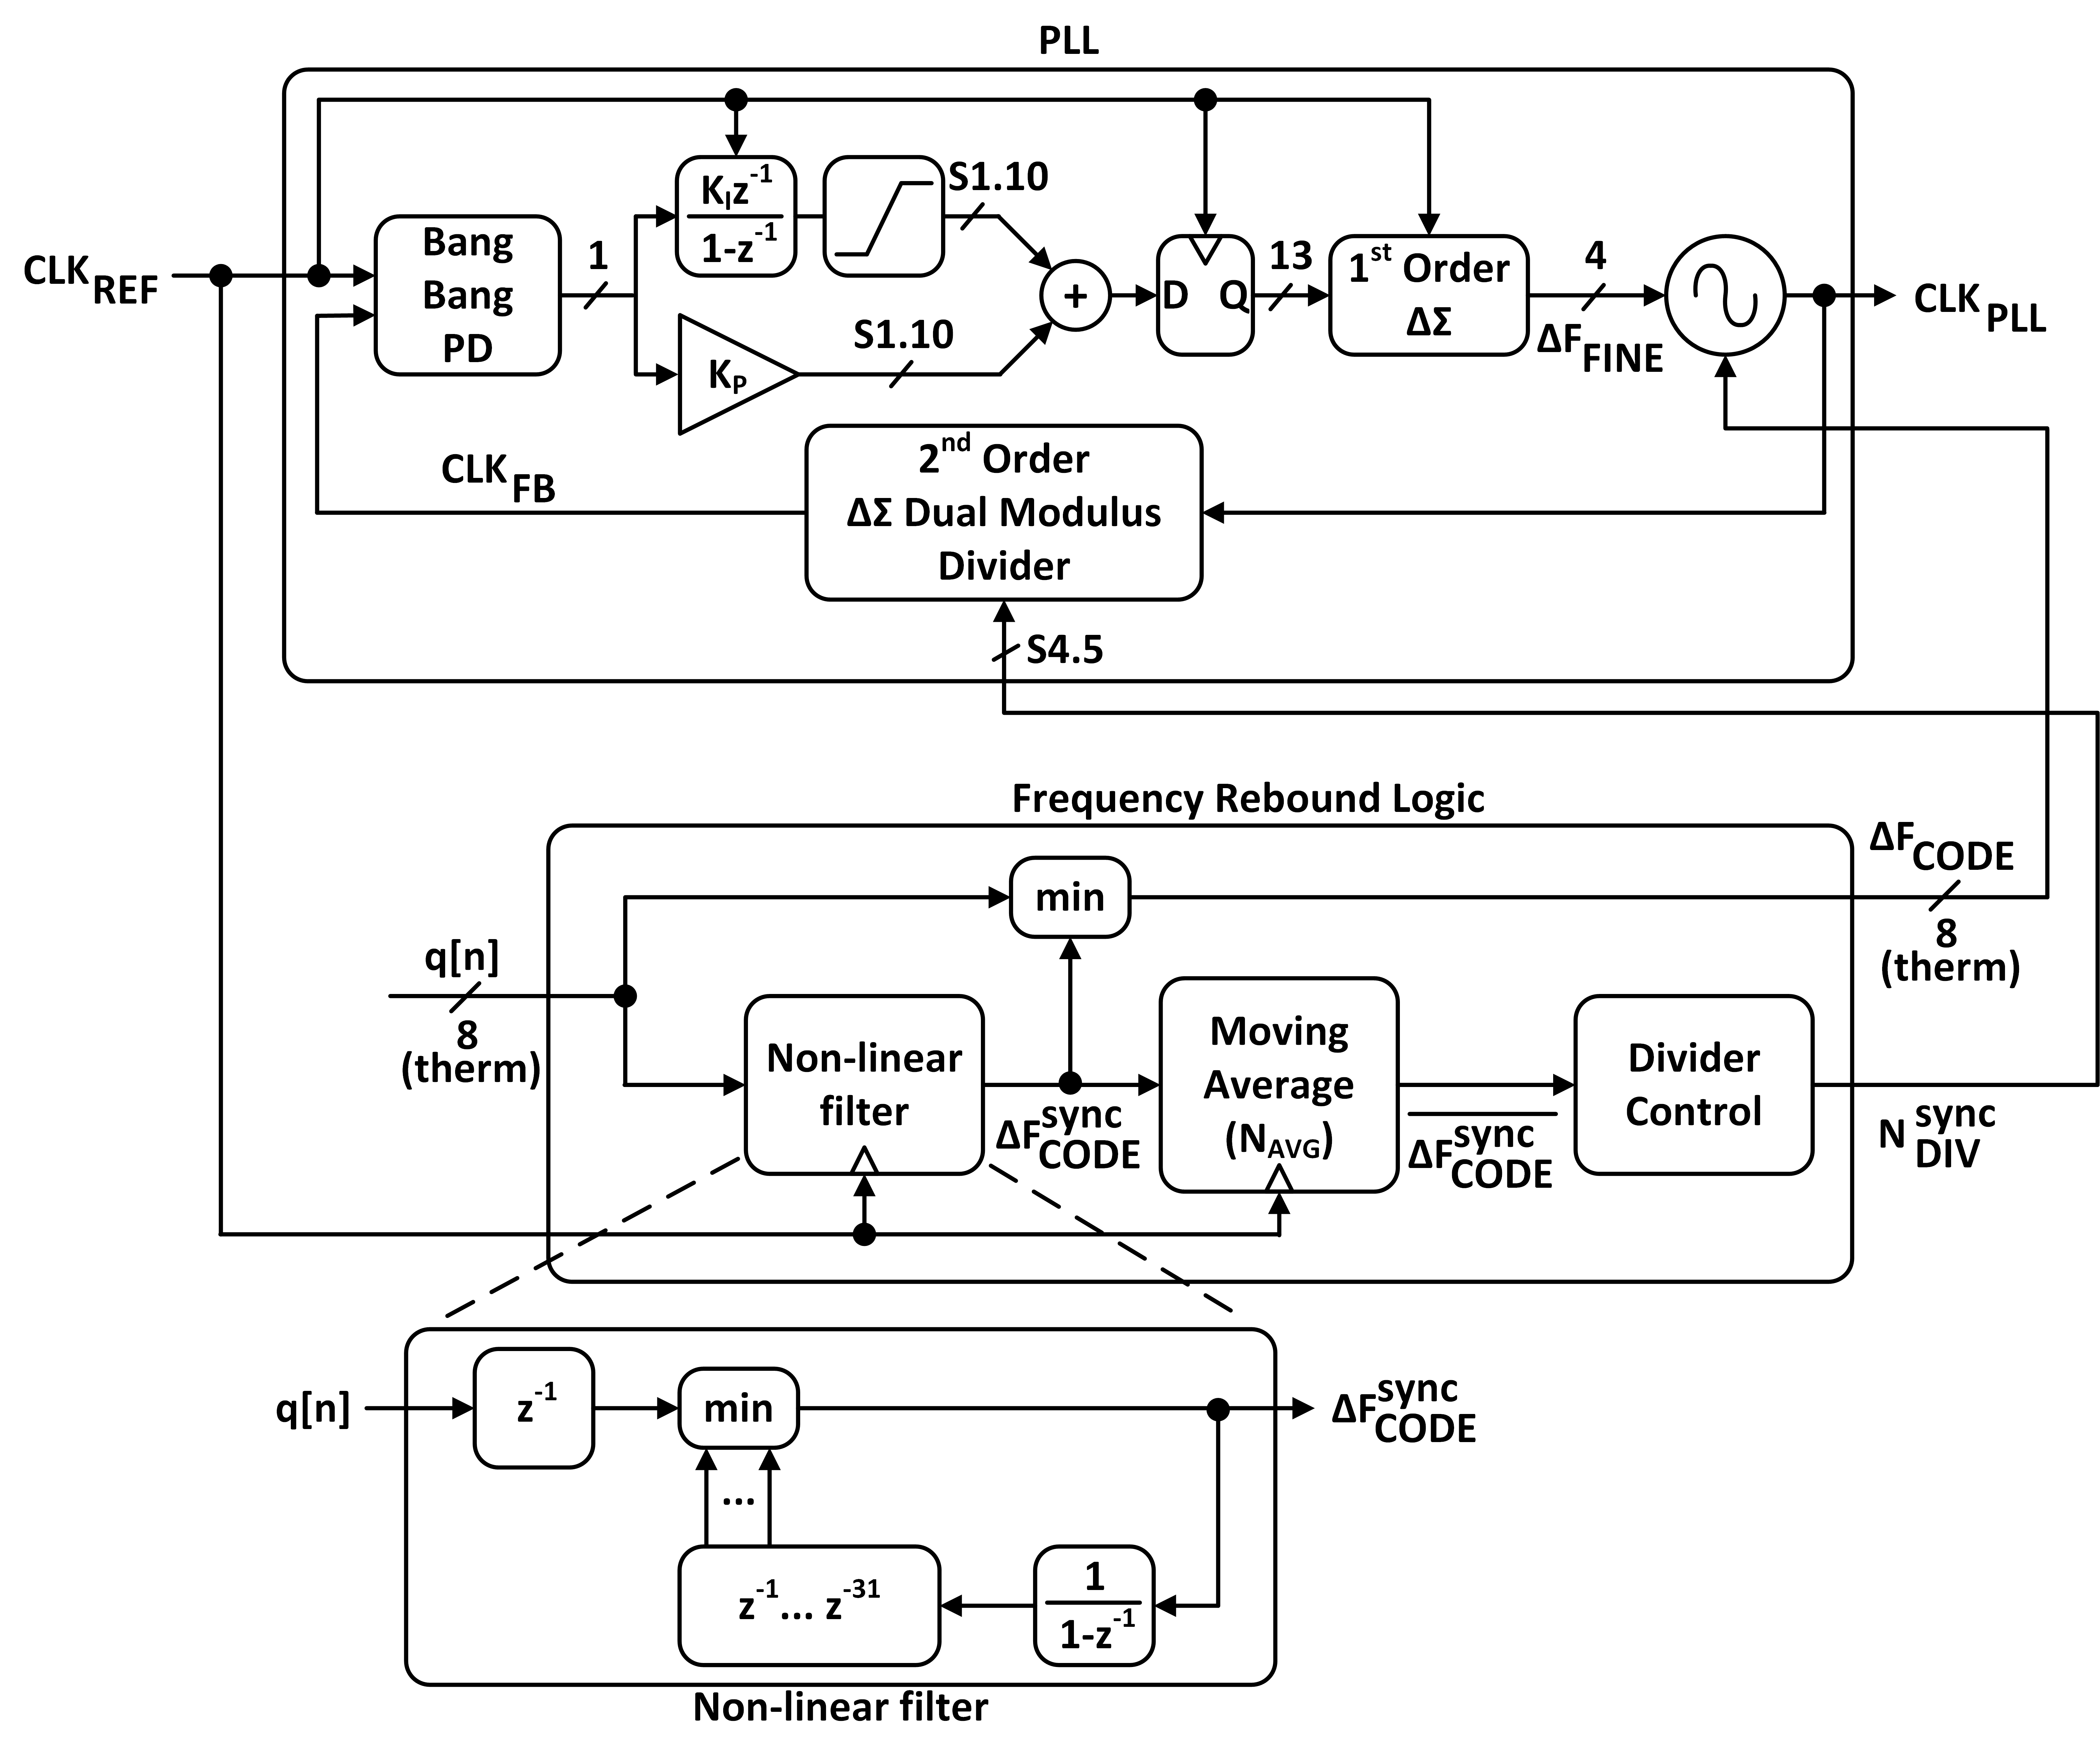
\includegraphics[width=\columnwidth]{fig_pll_model}
	\caption{Top-level implementation of PLL-based scheme from \cite{hashimoto2018}.}
	\label{fig:pll_model}
\end{figure}

The response to a droop event simulated in MATLAB is shown in Fig.\ \ref{fig:drooptransient}. The critical latencies from transistor-level simulations (Section \ref{sec:circuit_design}) are assumed. A short, maximum droop impulse is injected by q[n]. The frequency rebound controller then tunes $\Delta F_{CODE}$ that, after an actuation latency, directly changes the DCO frequency. The controller also slowly tunes the divider ratio to re-lock the PLL at the new DCO frequency and ramp the DCO back up to its nominal value. The PLL thereby recovers from the droop impulse after 540ns.

\vspace{-5pt}
\begin{figure}[h]
	\centering
	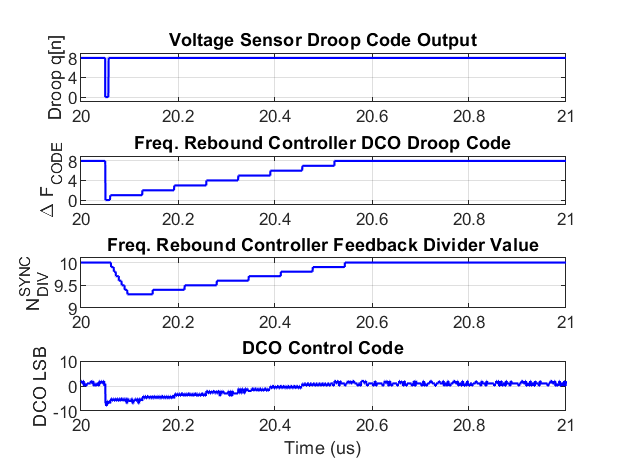
\includegraphics[width=\columnwidth]{fig_drooptransient}
	\caption{PLL and frequency control transient response to maximum droop.}
	\label{fig:drooptransient}
\end{figure}

\vspace{-3pt}
\subsection{Logic Design}
\label{sec:logic_design}

Save for the DCO and phase detector, the PLL was designed in IEEE1800-standard SystemVerilog. A parameterized phase-detector interface allows integration of the loop filter with either multi-bit TDCs or single-bit bang-bang PDs. The loop filter gains were also configurable. 

% -- WR: Already discussed above with figure.
%In addition to each of the conventional digital PLL sub-blocks (oscillator, detector, filter, and division), it includes a `DroopManager` component with a single primary input, `DroopDetected`, and primary outputs $\Delta F_{CODE}$ and $N_{DIV}^{sync}$. Each droop event incurs two discrete steps: response and recovery. During response, both $\Delta F_{CODE}$ and $N_{DIV}^{sync}$ are held at statically-programmable levels until `DroopDetected` is de-asserted for a parameterizable number of reference cycles. Droop-recovery then proceeds by simultaneously and coherently reducing $\Delta F_{CODE}$ and $N_{DIV}^{sync}$ towards zero. 

As discussed in \cite{hashimoto2018}, the frequency control logic latency must be minimized to reduce the overall droop actuation latency. To do so, the asynchronous $min$ path was thermometer-encoded logic to follow the implementation in \cite{hashimoto2018}. This reduces the propagation delay to a single AND logic gate plus associated wiring delays. The post-place-and-routed timing-annotated simulation, shown in Fig.\ \ref{fig:freqreboundctrl_postpandr_timing}, measures a 40ps latency through this path at the SS 0.63V $100^{\circ}$C corner. 

\vspace{-7pt}
\begin{figure}[h]
	\centering
	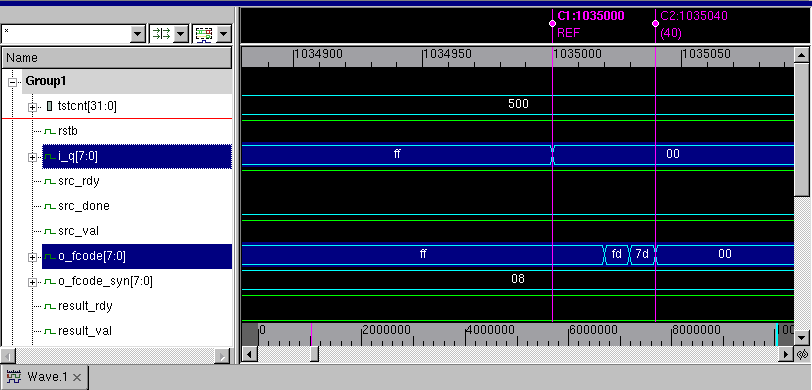
\includegraphics[width=\columnwidth]{fig_freqreboundctrl_postpandr_timing}
	\caption{Post-place-and-route timing-annotated simulation of input to output delay in frequency rebound logic ($q[n]$ to $\Delta F_{CODE}$ at SS corner).}
	\label{fig:freqreboundctrl_postpandr_timing}
\end{figure}
\vspace{-5pt}

PLL lock is achieved through a three-step process: coarse frequency calibration, fine phase locking, and droop response. The latter two interactions have been discussed and demonstrated above. The coarse frequency calibration, conducted to initially bring the DCO within the PLL frequency capture range, sets the DCO's coarse oscillator code. The nominal coarse step is 250MHZ/LSB. This code is frozen following coarse lock, after which point the PLL assumes phase locking control through the fine DAC. The segmentation of the coarse and fine DACs are discussed in \ref{sec:circuit_design}. 

% WR -- Already discussed/shown in system-level.
%During a droop event, a combination of the oscillator's linearity requirements and offline calibration data enable the PLL frequency to change to near exactly its target frequency instantaneously. Imprecision and/or quantization in this calibration data, coupled with runtime oscillator shifts (again likely due to temperature) generally cause a small frequency error, which the PLL loop then removes. During such frequency shifts, phase lock is generally lost. Digital PLLs commonly maintain loss-of-lock detection schemes which observe an error variable in the PLL state (e.g. the phase detector output), and declare loss-of-lock when these variables exceed predetermined thresholds. To maintain such protections while enabling lock through droop events, the PLL uses its fine-frequency mode throughout droop response and recovery. 

A sample RTL simulation in Fig.\ \ref{fig:brake} shows the PLL initially locking to a target $f_{DCO}$ of 4.0GHz, then responding to a droop event and temporarily reducing its frequency to 3.5GHz before recovering and restoring DCO frequency.

\begin{figure}[h]
	\centering
	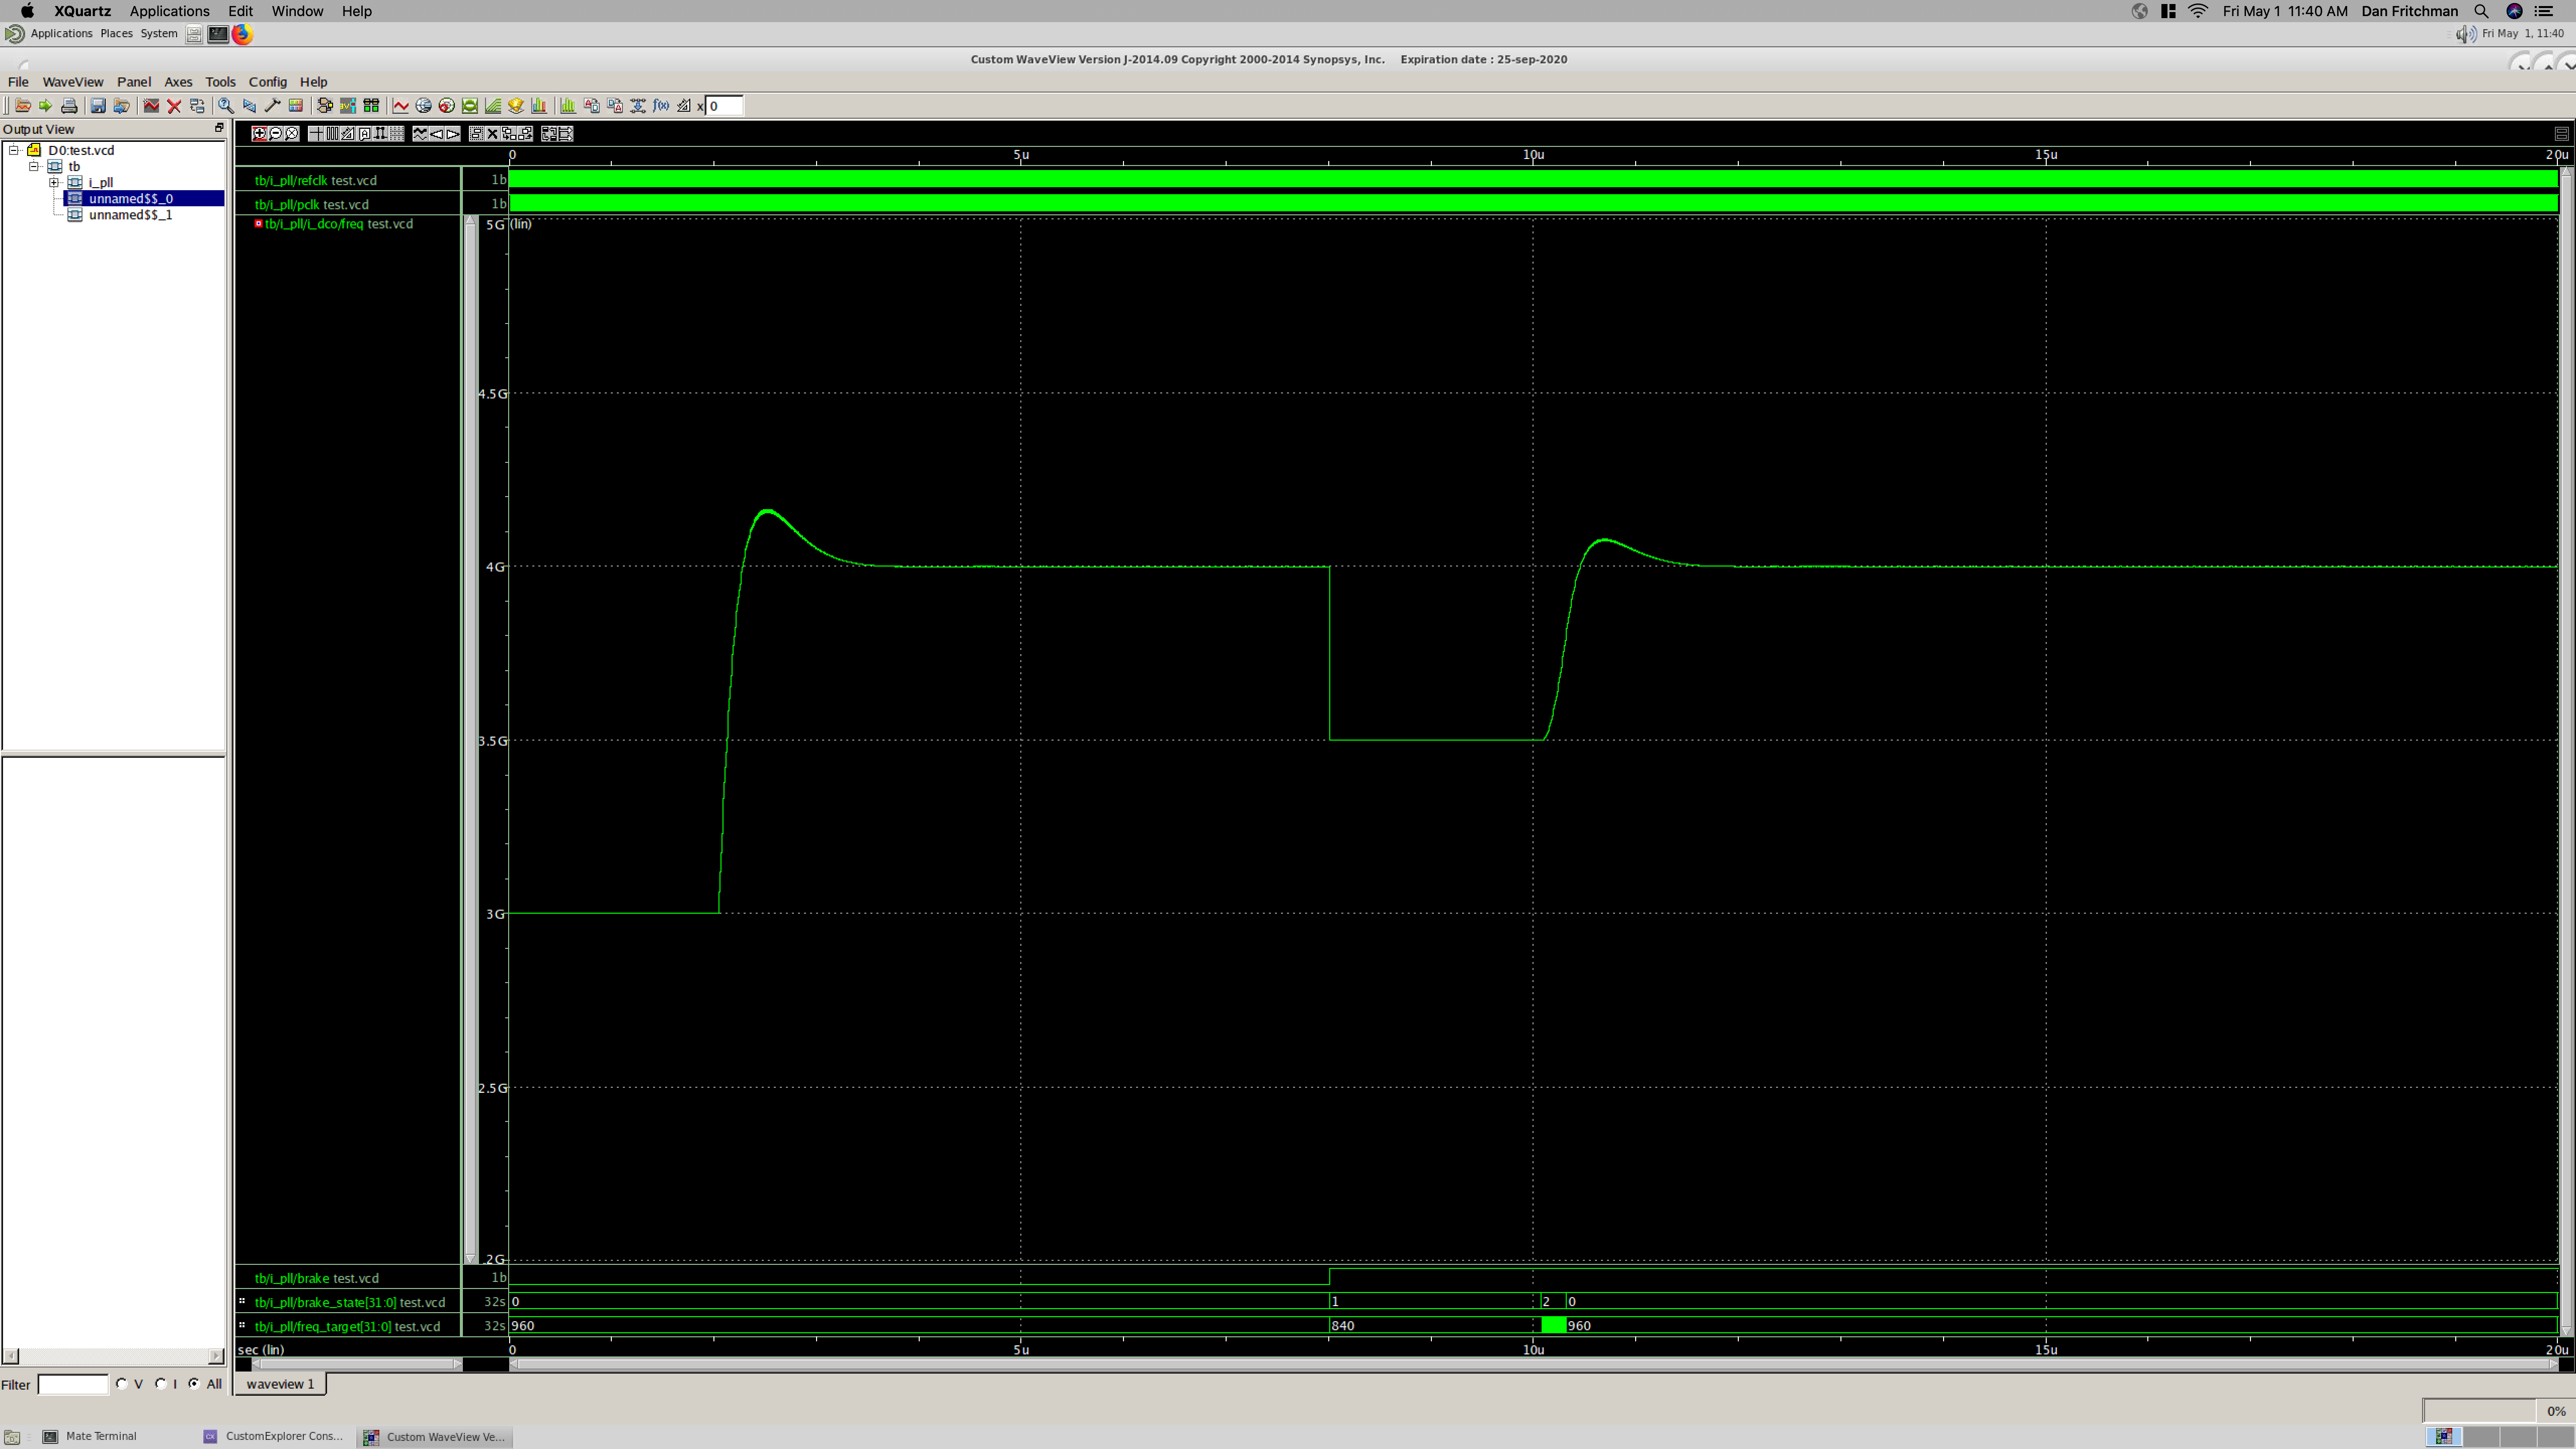
\includegraphics[width=\columnwidth]{brake1.png}
	\caption{Logic simulation of initial lock, droop response, and droop recovery from 4.0GHz to 3.5GHz and back to 4.0GHz. Main waveform shows DCO frequency vs. time.}
	\label{fig:brake}
\end{figure}

\vspace{-7pt}
\subsection{Circuit Design and Implementation}
\label{sec:circuit_design}

The PLL layout, generated by standard EDA tools and the HAMMER \cite{wanghammer} back-end toolchain, is shown in Fig.\ \ref{fig:layout}. Its area is 10,000 $\mu m^2$ (100$\mu m$$\times$100$\mu m$). This figure excludes the custom-designed DCO, which was estimated to comprise 100$\mu m^2$ or less than 1\% of the overall PLL area.

\begin{figure}[h]
	\centering
	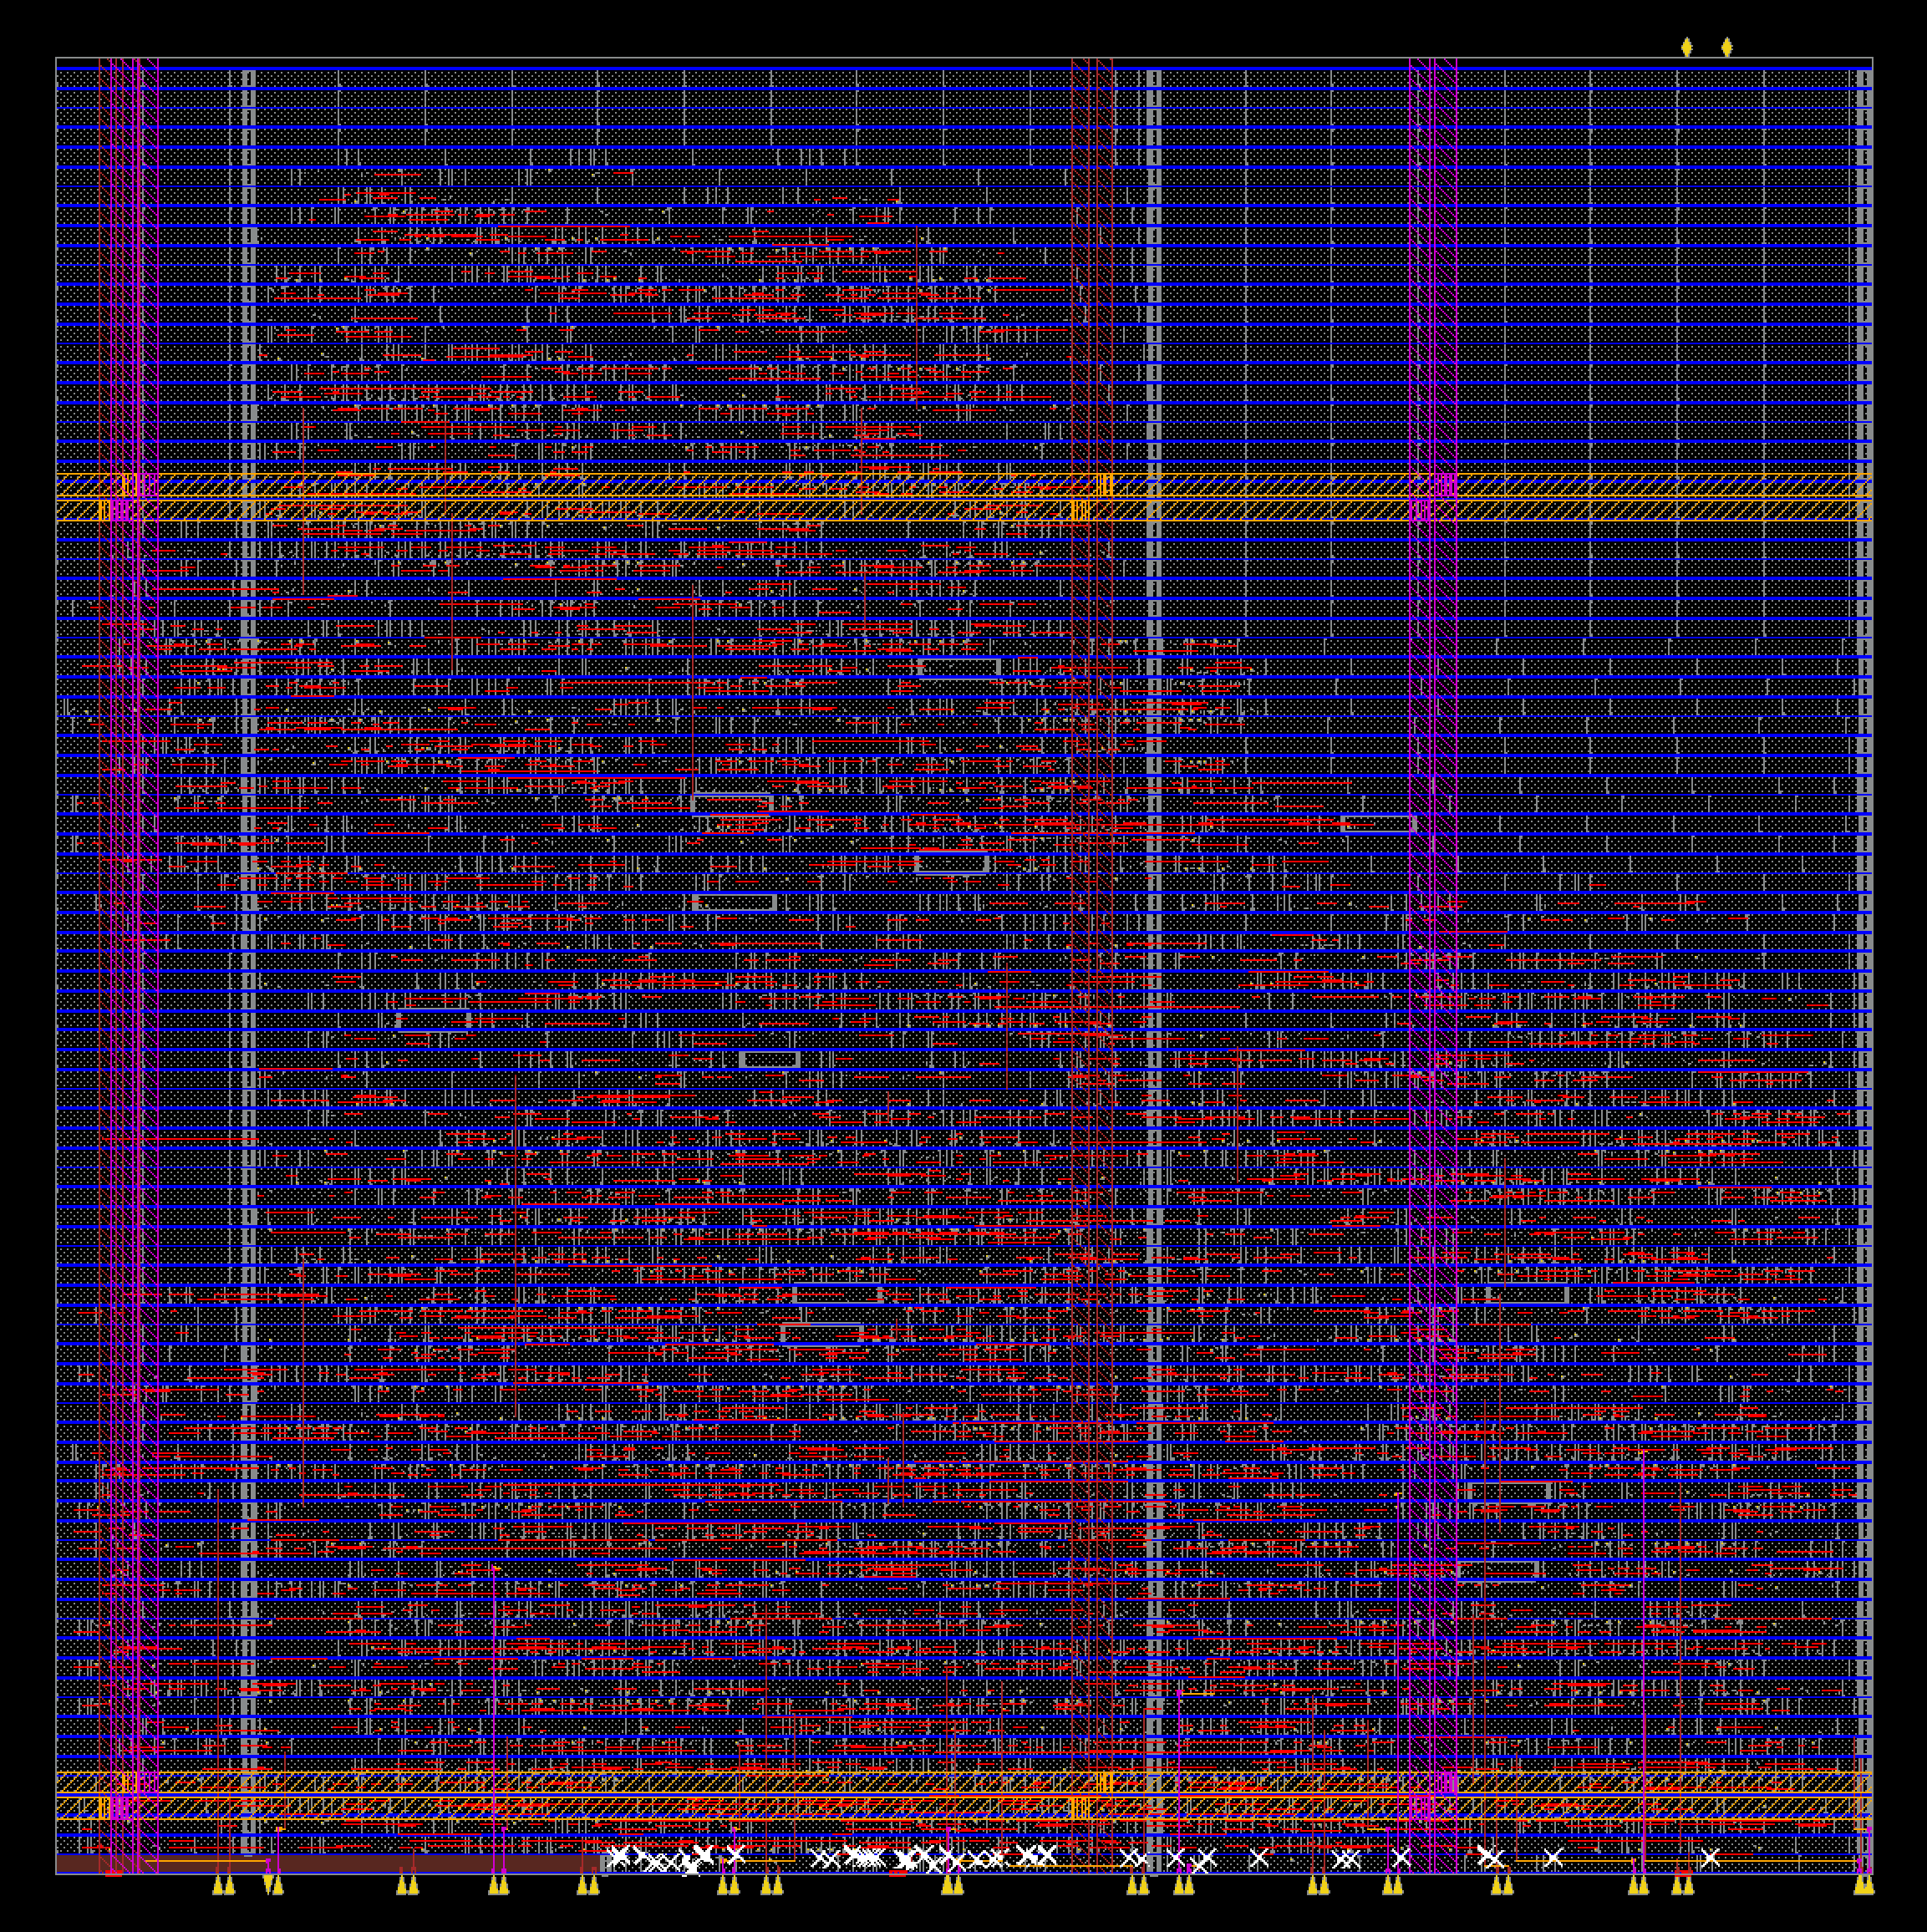
\includegraphics[width=0.7\columnwidth]{pnr3.png}
	\caption{PLL layout in ASAP7 predictive technology (100$\mu m\times100\mu m$). DCO is omitted.}
	\label{fig:layout}
\end{figure}

The top-level DCO schematic, shown in Fig.\ \ref{fig:dco}, was simulated with cell-level RC extractions using Calibre and 60fF of estimated wire capacitances added to each node. For this prototype design, the $CLK_{DCO}$ was chosen to have an $f_{MAX}$ of 5GHz to match the reported $f_{MAX}$ in \cite{hashimoto2018}. This PLL was designed with a $CLK_{REF}$ frequency of 500MHz and a nominal division ratio $N_{DIV}^{sync}$ of 10. The DCO consisted of custom C2MOS cells as shown in Fig.\ \ref{fig:c2mos}. 

\begin{figure}[h]
	\centering
	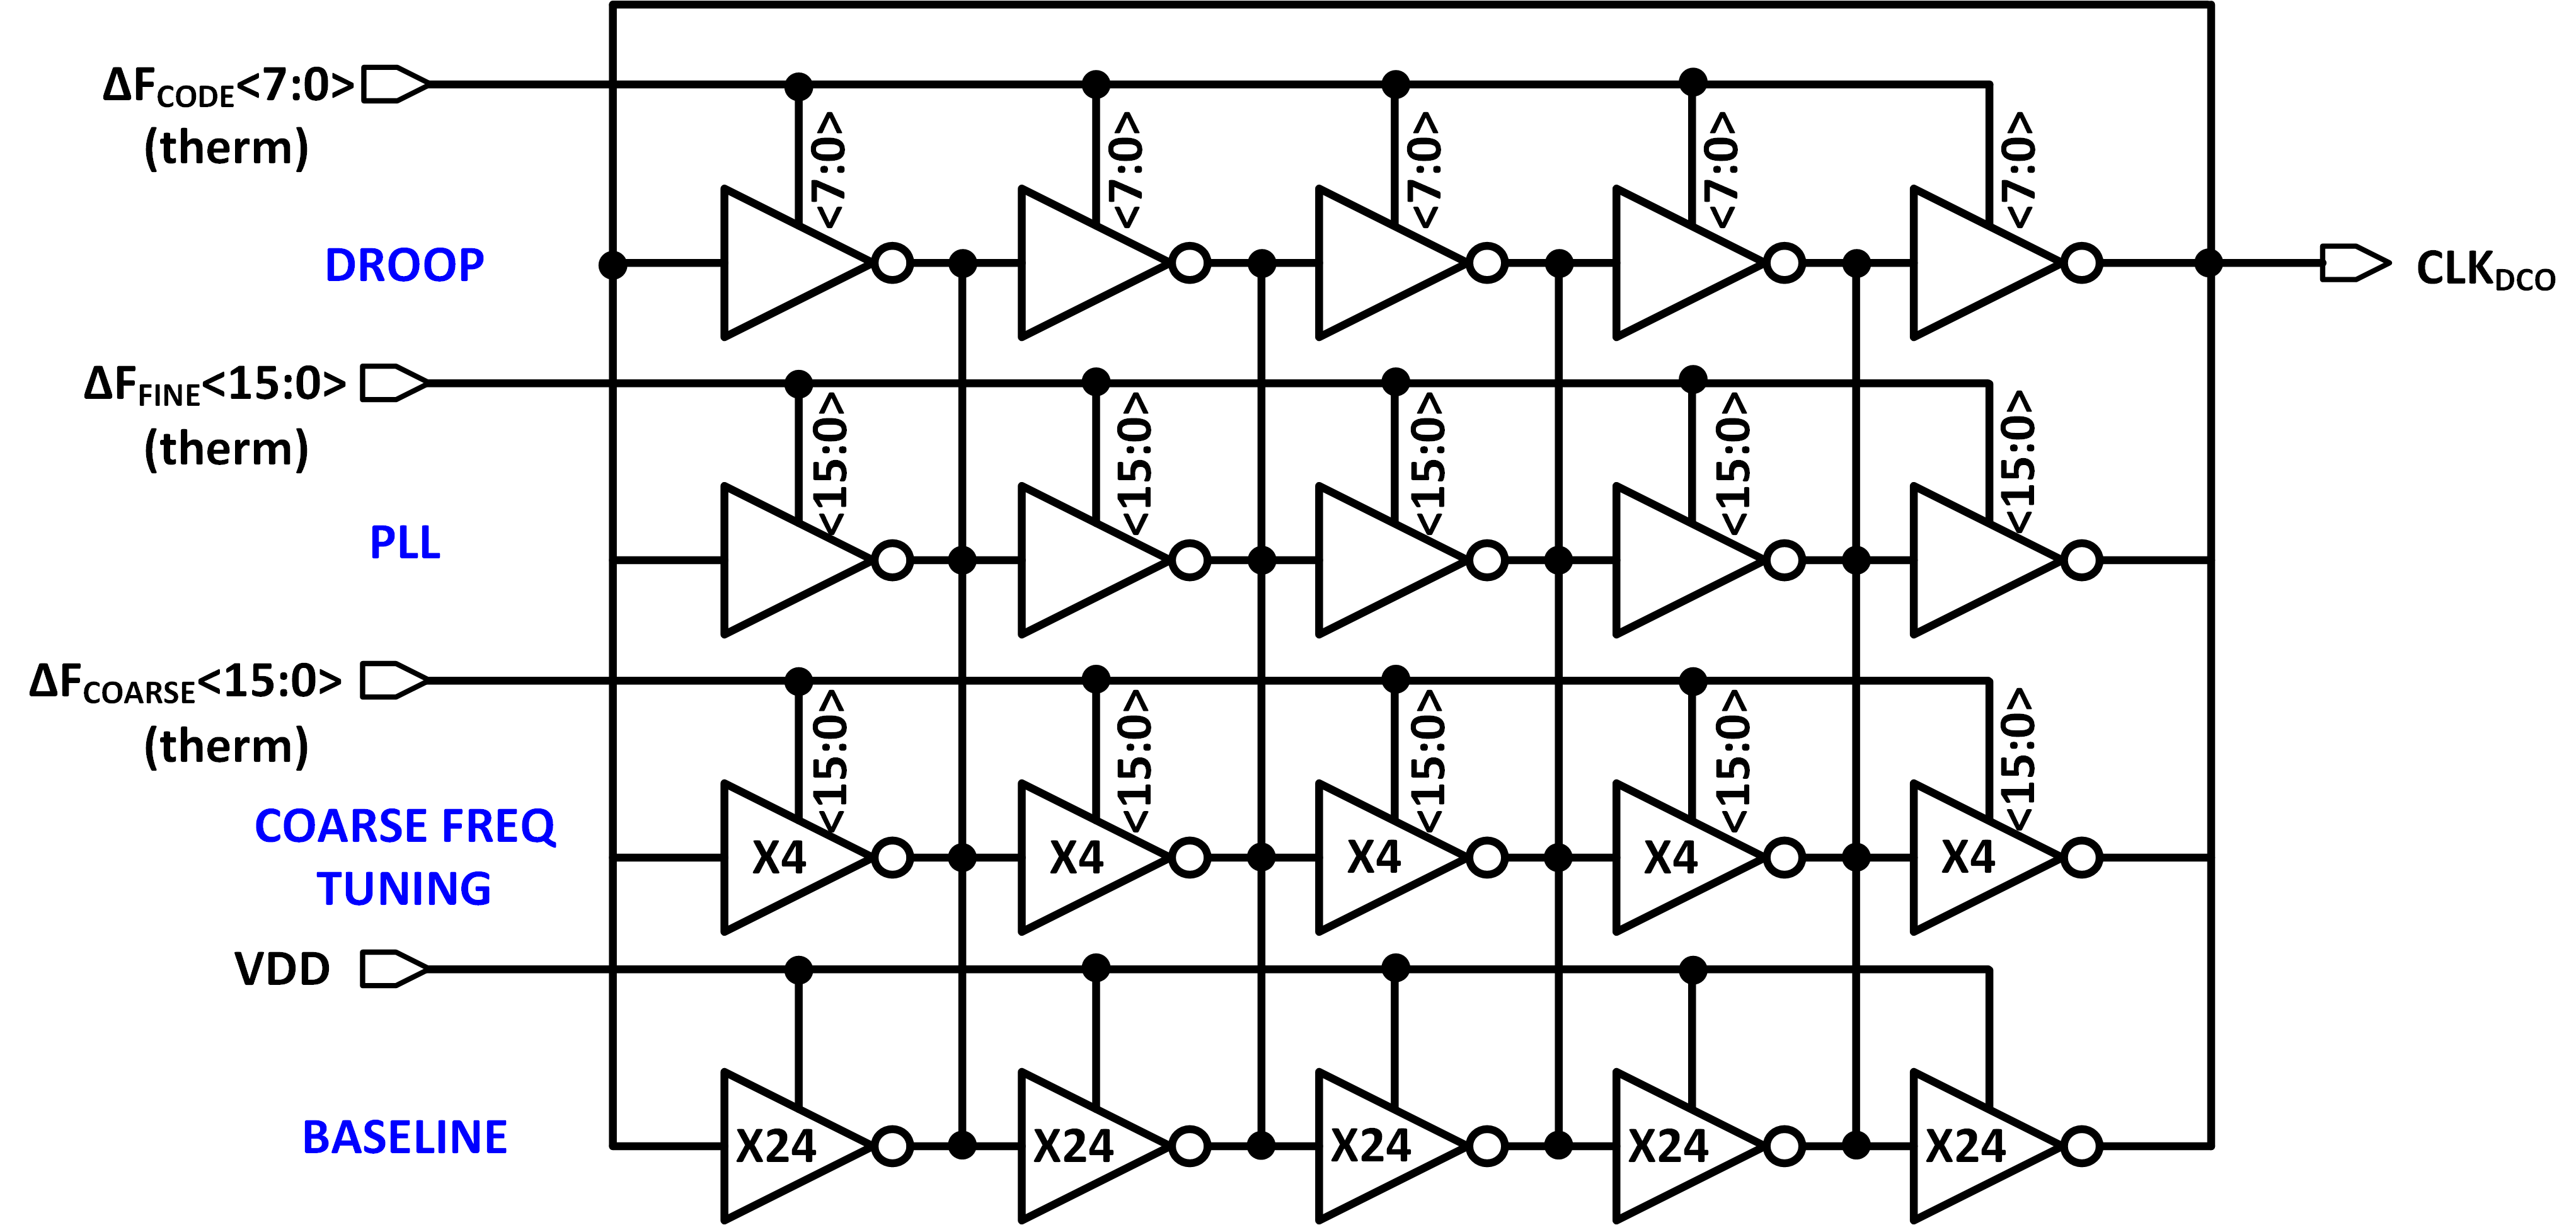
\includegraphics[width=0.9\columnwidth]{fig_dco}
	\caption{DCO schematic using custom C2MOS cells.}
	\label{fig:dco}
\end{figure}

\begin{figure}[h]
	\centering
	\begin{minipage}{0.49\columnwidth}
	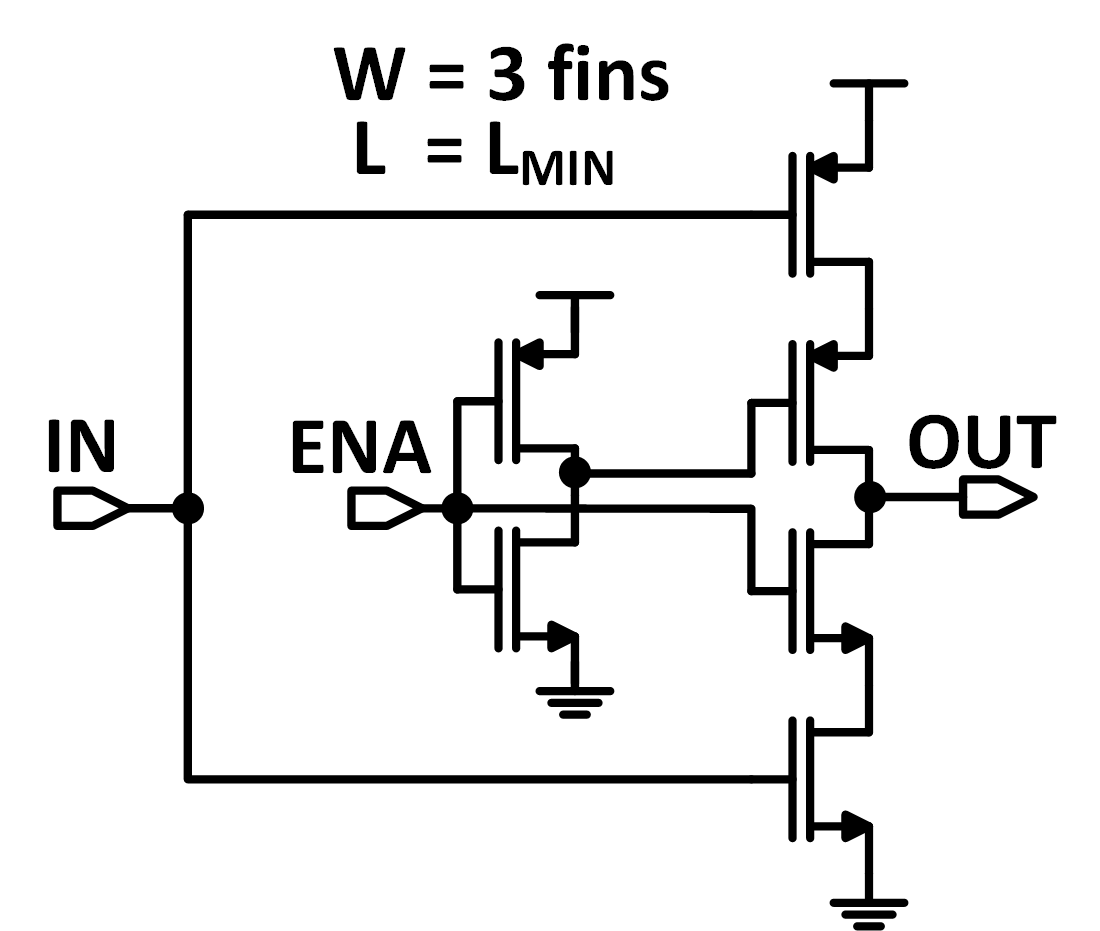
\includegraphics[width=\textwidth]{fig_c2mossch}
	%\caption{Custom C2MOS schematic.}
	\end{minipage}
	\hfill
	\begin{minipage}{0.49\columnwidth}
	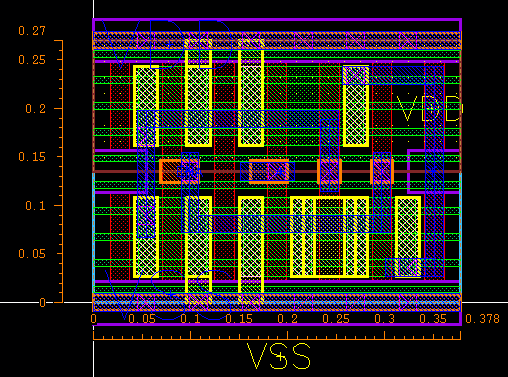
\includegraphics[width=\textwidth]{fig_c2moslayout}
	%\caption{Custom C2MOS layout.}
	\end{minipage}
	\caption{Custom C2MOS schematic and layout for DCO implementation.}
	\label{fig:c2mos}
\end{figure}

The design objective was to achieve an octave (2:1) frequency tuning range across corners with sufficiently small resolution for PLL dynamics. This was achieved with segmented coarse- and fine DACs. The fine DAC was designed to span approximately four coarse LSBs: even after initial frequency calibration froze the coarse codes, the PLL could span that range through the fine DAC if lock dynamics required. This segmentation then obviates gain calibration between the two DACs. For brevity, tuning curves for only the typical corner are shown in Fig.\ \ref{fig:dco_oscctrl}.

\vspace{-10pt}
\begin{figure}[h]
	\centering
	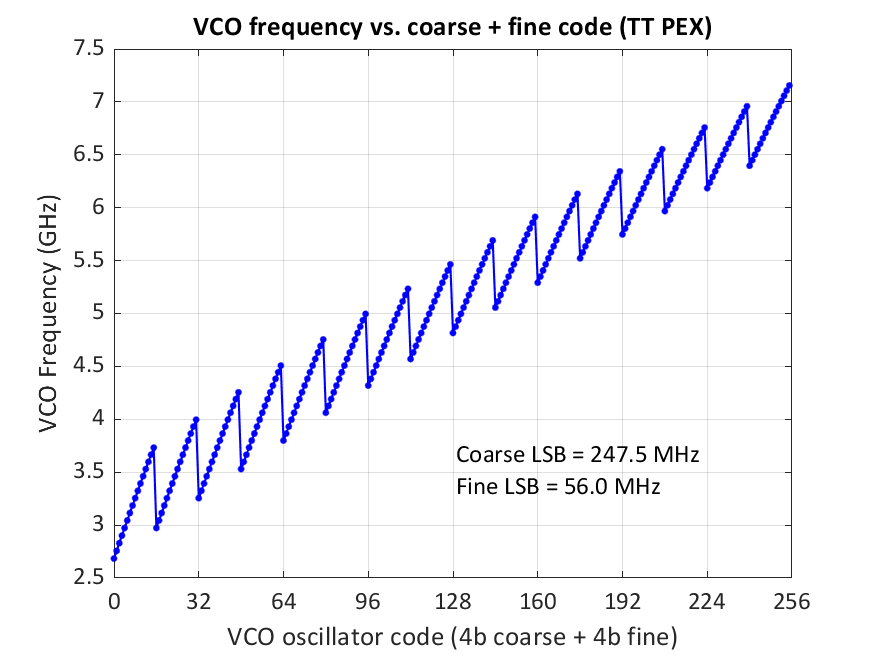
\includegraphics[width=0.7\columnwidth]{fig_dco_oscctrl}
	\caption{DCO frequency vs. coarse + fine DAC code at TT corner.}
	\label{fig:dco_oscctrl}
\end{figure}

The smaller droop control DAC was designed to tolerate a 10\% change in frequency at an $f_{MAX}$ of 5GHz. At high $V_{DD}$, this corresponds to roughly a 10\% droop in supply, corresponding to the maximum droop transient shown previously in Fig.\ \ref{fig:droop}. Eight thermometer bits were used for the total droop range, mapping to 60MHz/LSB. The response of this droop control is shown in Fig.\ \ref{fig:dco_droopctrl}.

\vspace{-10pt}
\begin{figure}[h]
	\centering
	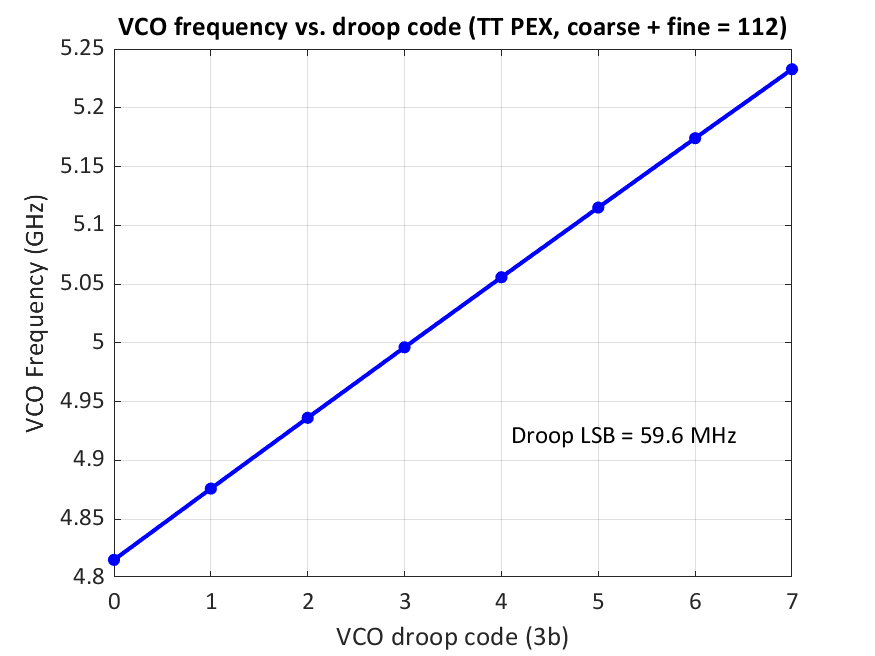
\includegraphics[width=0.7\columnwidth]{fig_dco_droopctrl}
	\caption{DCO frequency vs. droop code at TT corner (coarse + fine centred at 5GHz).}
	\label{fig:dco_droopctrl}
\end{figure}
\vspace{-5pt}

The actuation time of the droop input control of the DCO to the time the DCO output clock frequency settles in frequency is shown in Fig.\ \ref{fig:dco_response} for TT corner and extracted C2MOS cells. For a full-scale change at the droop input requires 267ps to settle to the new frequency, or $6.675\times$ higher than the frequency control logic latency of 40ps reported in Section \ref{sec:logic_design}.

\vspace{-10pt}
\begin{figure}[h]
	\centering
	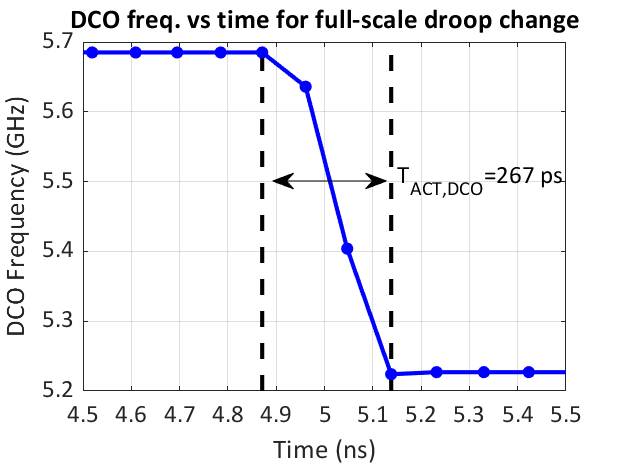
\includegraphics[width=0.7\columnwidth]{fig_dco_response}
	\caption{DCO frequency vs. time with full-scale DCO droop code change.}
	\label{fig:dco_response}
\end{figure}

\section{Discussion}
\label{sec:discussion}
\subsection{Actuation Latency Penalty to $f_{MAX}$}
\label{sec:actuation_latency}
As previously discussed, actuation latency is the time delay from a supply droop to the the clock frequency change. This serves as a proxy to evaluate how $f_{MAX}$ is improved by an adaptive clocking technique for an SoC. More precisely, consider the droop example illustrated in Fig.\ \ref{fig:drooptransient}. A supply droop occurs where $V_{DD}$ suddenly decreases from its ideal 1.0V, and the adaptive clocking technique adjusts SoC clock frequecy $f_{CLK}$ after actuation latency $T_{ACT}$. To mitigate timing failure during this latency, the SoC $f_{MAX}$ can only operate assuming $V_{DD,ACT}$, the supply voltage at the time $f_{CLK}$ changes. Actuation latency limits SoC performance.

\vspace{-7pt}
\begin{figure}[h]
	\centering
	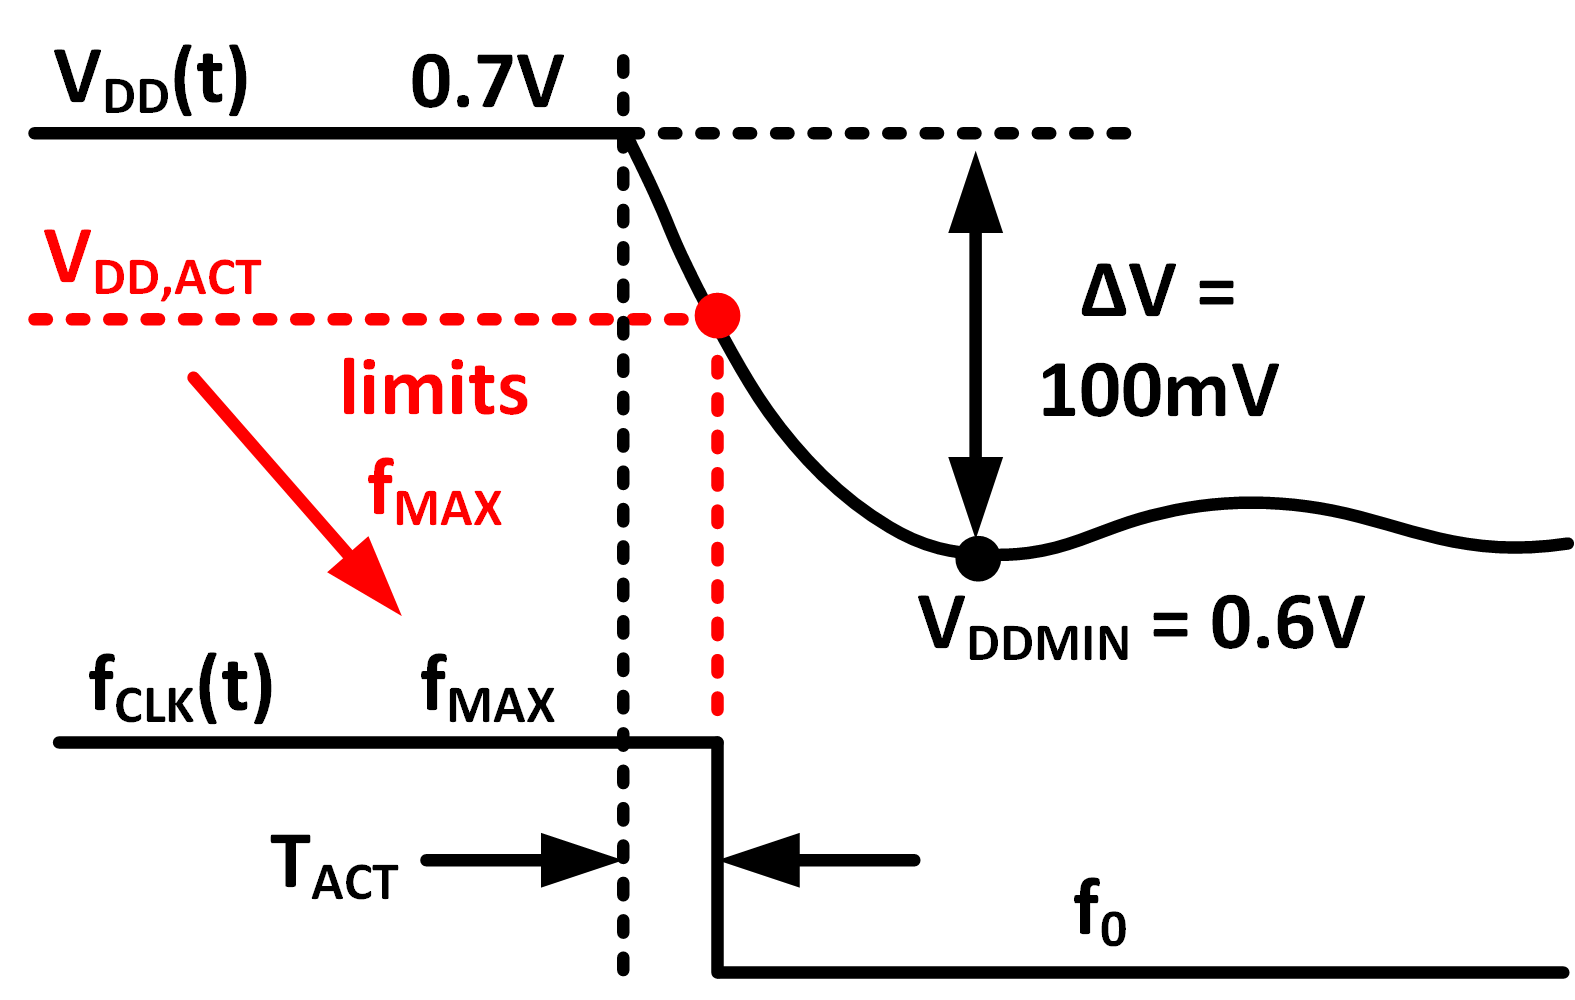
\includegraphics[width=0.6\columnwidth]{fig_drooplatency}
	\caption{Effect of droop activation latency on $f_{MAX}$.}
	\label{fig:drooplatency}
\end{figure}

If the supply voltage initially follows $V_{DD}(t) = -\Delta V_{d}sin(2\pi f_{d}t)$ from the linear $RLC$ supply network, where $\Delta V_{d}$ and $f_{d}$ are the voltage drop and frequency of the worst-case droop, then the slope of $V_{DD}(t)$ near the start of the droop is $-2\pi \Delta V_{d}f_{d}$. Using $T_{ACT}$, it can be shown that $V_{DD,ACT} = V_{DD}-2\pi \Delta V_{d}f_{d}T_{ACT}$. Assuming high $V_{DD}$ and a linear transistor model, the achievable $f_{MAX}$ is:

\begin{equation}
\label{eq:fmax_penalty}
f_{MAX} = (1 - \frac{2\pi\Delta V_{d}f_{d}}{V_{DD}}T_{ACT})f_{MAX,ideal}
\end{equation} 
where $f_{MAX,ideal}$ is the maximum SoC clock frequency when $V_{DD}$ is at its maximum voltage. It is apparent from Eq.\ \ref{eq:fmax_penalty} that, to minimize impact on performance, either the actuation latency, droop voltage, or droop frequency must be reduced or the nominal supply voltage must be increased. In ASAP7 for example, the simulated logic \& DCO latencies total $T_{ACT}$ = 40ps + 267ps = 307ps and $V_{DD}$ = 0.7V nominally. To target a 100mV first droop with 50MHz ripple as in \cite{hashimoto2018}, a 1.4\% $f_{MAX}$ penalty is incurred from $f_{MAX,ideal}$. Note that clock tree insertion delay can significantly change this: simulated delays in ASAP7 for a chain of 45 FO4 inverters incur a delay of 951ps, increasing $T_{ACT}$ to 938ps and thus $f_{MAX}$ penalty to 5.6\%.

\vspace{-5pt}
\subsection{Comparison to Prior Works}
\label{sec:comp-priors}
Table \ref{table:comparison} shows a comparison of this feasibility study with prior works discussed. A key point in the analysis from Eq.\ \ref{eq:fmax_penalty} above is that prior works do not report the theoretical $f_{MAX,ideal}$, but only the comparisons between $f_{MAX}$ achieved with and without their reported adaptive clocking schemes. This includes clock tree insertion delay, which may dominate $T_{ACT}$ and thus the $f_{MAX}$ penalty.

\begin{table}[!ht]
\caption{Comparison to Prior Works} 
\label{table:comparison}
\centering
\begin{tabularx}{\columnwidth}{
	| >{\centering\arraybackslash}X 
	| >{\centering\arraybackslash}X 
	| >{\centering\arraybackslash}X 
	| >{\centering\arraybackslash}X | }
	\hline
	& \cite{wilcox2015} & \cite{hashimoto2018} & This work \\
	\hline
	Process & 28nm CMOS & 20nm CMOS & 7nm Predictive CMOS  \\
	\hline
	Detection Method & Droop sensor & Droop sensor & Droop sensor (assumed)  \\
	\hline
	Adaptation Method & DLL \& Phase Rotator & Adaptive PLL & Adaptive PLL  \\
	\hline
	Logic Latency & 588ps & 200ps & 40ps  \\
	\hline
	Clock Freq. Latency & 294ps (phase rotator) & Not reported & 267ps (DCO)  \\
	\hline
	Power & Not reported & Not reported & 1.65mW (DCO only) \\
	\hline
	Area & Not reported & Not reported & 10,100 $\mu m^2$ \\
	\hline
\end{tabularx}
\end{table}

The prototype implemented here based on \cite{hashimoto2018} suggests that design is indeed feasible in ASAP7: as Table \ref{table:comparison} shows, ASAP7 achieves a $5\times$ lower logic latency in the frequency rebound controller from \cite{hashimoto2018}. However, the reported benefits of low-latency frequency rebound control logic is likely small. The DCO actuation time was 267ps in this study: the logic latency accounted for only 15\% of the total $T_{ACT}$ even before clock tree insertion. While \cite{hashimoto2018} does not report their DCO latency, logic latency plays an increasingly small role compared to other clocking latencies in ASAP7. Future research can incorporate DCO actuation and clock insertion latencies to achieve a lower effective $T_{ACT}$ and a lower $f_{MAX}$ penalty from ideal.

\vspace{-5pt}
\section{Conclusion}
\label{sec:conclusion}

This work compares the costs and effectiveness of ACD- and PLL-based adaptive clocking systems \cite{hashimoto2018,wilcox2015}. ACD-based systems exchange design complexity for higher power and area, but both systems achieve low-latency actuation and performance. To study feasibility in FinFET, the PLL-based system was implemented in a predictive 7nm CMOS, reporting power, area, and a $5\times$ lower detection logic latency. However, other delays such as the DCO and clock distribution dominate the overall actuation latency, and a theoretical penalty is presented. Both suggest that further FinFET speed-ups in detection logic will have diminishing returns; adaptive clocking systems must consider other latencies in the overall design. 

\vspace{-5pt}
\bibliographystyle{IEEEtran}
\begingroup
\raggedright
\bibliography{references}
\endgroup

\end{document}
